\documentclass[9pt, aspectratio=169]{beamer}
% \documentclass[10pt]{beamer}
\usepackage[utf8]{inputenc}
\usepackage[T1]{fontenc}
\usepackage[english]{babel}
\usetheme{Frankfurt}

\usepackage[backend=biber, style=authoryear]{biblatex}
\addbibresource{local_references.bib}

%\usepackage{lmodern}
\usepackage{amsfonts,amssymb,amsmath}
\usepackage[english]{babel}
\usetheme{Frankfurt}

\usepackage{csquotes}
\usepackage{setspace}

\usepackage{colortbl}
\usepackage{tabularx}
\renewcommand\tabularxcolumn[1]{m{#1}}

% --- Tickz
\usepackage{physics}
\usepackage{amsmath}
\usepackage{tikz}
\usepackage{mathdots}
\usepackage{yhmath}
\usepackage{cancel}
\usepackage{color}
\usepackage{siunitx}
\usepackage{array}
\usepackage{multirow}
\usepackage{amssymb}
\usepackage{gensymb}
\usepackage{tabularx}
\usepackage{extarrows}
\usepackage{booktabs}
\usetikzlibrary{fadings}
\usetikzlibrary{patterns}
\usetikzlibrary{shadows.blur}
\usetikzlibrary{shapes}

% ---------

\usepackage{booktabs}
\usepackage{setspace}
\usepackage{amssymb}
\usepackage{adjustbox}
\usepackage{pifont}
\usepackage[inkscapeformat=png]{svg}
\usepackage{graphicx}
\usepackage{times}
\setbeamertemplate{caption}[numbered]
% % \setbeamertemplate{bibliography item}{[\theenumiv]}

\setbeamerfont{bibliography item}{size=\tiny}
\setbeamerfont{bibliography entry author}{size=\tiny}
\setbeamerfont{bibliography entry title}{size=\tiny}
\setbeamerfont{bibliography entry location}{size=\tiny}
\setbeamerfont{bibliography entry note}{size=\tiny}

\setbeamerfont{frametitle}{size=\large}

\usepackage{caption}
\usepackage{float}
\usepackage{xcolor}
\usepackage{listings}
\usepackage{animate}

\definecolor{codegreen}{rgb}{0,0.6,0}
\definecolor{codegray}{rgb}{0.5,0.5,0.5}
\definecolor{codepurple}{rgb}{0.58,0,0.82}
\definecolor{backcolour}{rgb}{0.95,0.95,0.92}
 
\lstdefinestyle{mystyle}{
    backgroundcolor=\color{backcolour},   
    commentstyle=\color{codegreen},
    keywordstyle=\color{magenta},
    numberstyle=\tiny\color{codegray},
    stringstyle=\color{codepurple},
    basicstyle=\footnotesize,
    breakatwhitespace=false,         
    breaklines=true,                 
    captionpos=b,                    
    keepspaces=true,                 
    numbers=left,                    
    numbersep=5pt,                  
    showspaces=false,                
    showstringspaces=false,
    showtabs=false,                  
    tabsize=2
}
 
\lstset{style=mystyle}

\usepackage{ragged2e}
\setbeamercolor{section in foot}{fg=white,bg=darkorange}
\setbeamercolor{subsection in foot}{fg=white,bg=darkorange}
\setbeamercolor{frametitle}{fg=white, bg=darkorange}
\setbeamercolor{title}{fg=white, bg=darkorange}
\setbeamercolor{frame}{bg=darkorange}
\setbeamercolor{block title}{bg=darkorange,fg=white}

\setbeamercolor{item}{fg=darkorange}

% \definecolor{darkorange}{rgb}{0.81, 0.52, 0.05}
\definecolor{darkorange}{rgb}{1,0.5,0}
\definecolor{darkorange2}{rgb}{1, 0.64, 0.2}
\definecolor{honeydew}{rgb}{1, 0.85, 0.45}


\newenvironment{variableblock}[3]{%
  \setbeamercolor{block body}{#2}
  \setbeamercolor{block title}{#3}
  \begin{block}{#1}}{\end{block}}

\newenvironment{prosblock}[1]{%
  % \setbeamercolor{block body}{bg=blue,fg=white}
  \setbeamercolor{block title}{bg=blue,fg=white}
  \begin{block}{#1}}{\end{block}}

\newenvironment{consblock}[1]{%
  % \setbeamercolor{block body}{bg=red,fg=white}
  \setbeamercolor{block title}{bg=red,fg=white}
  \begin{block}{#1}}{\end{block}}

\newcommand{\cmark}{\ding{51}}%
\newcommand{\xmark}{\ding{55}}%

\renewcommand{\arraystretch}{1.5}

% Please add the following required packages to your document preamble:
\usepackage{booktabs}
\usepackage{multirow}
\usepackage{colortbl}
% Beamer presentation requires \usepackage{colortbl} instead of \usepackage[table,xcdraw]{xcolor}

\usepackage{tabularray}\UseTblrLibrary{varwidth}
\usepackage{xcolor}
\def\BibTeX{{\rm B\kern-.05em{\sc i\kern-.025em b}\kern-.08em
    T\kern-.1667em\lower.7ex\hbox{E}\kern-.125emX}}
% \usepackage{cite}
\usepackage{amsmath}
\newcommand{\probP}{\text{I\kern-0.15em P}}
\usepackage{etoolbox}
\patchcmd{\thebibliography}{\section*{\refname}}{}{}{}

\setlength\tabcolsep{0.5pt}

\renewcommand{\arraystretch}{0.9}
\setlength{\tabcolsep}{2pt}

\usepackage{pgffor}
\usepackage[absolute,overlay]{textpos}
\setlength{\TPHorizModule}{1cm}
\setlength{\TPVertModule}{1cm}

\setbeamerfont{bibliography item}{size=\tiny}
\setbeamerfont{bibliography entry author}{size=\tiny}
\setbeamerfont{bibliography entry title}{size=\tiny}
\setbeamerfont{bibliography entry location}{size=\tiny}
\setbeamerfont{bibliography entry note}{size=\tiny}

\setbeamerfont{bibliography entry author}{shape=\upshape,series=\mdseries,size=\footnotesize}
\setbeamerfont{bibliography entry title}{shape=\slshape,series=\mdseries,size=\footnotesize}
\setbeamerfont{bibliography entry journal}{shape=\upshape,series=\mdseries,size=\footnotesize}
\setbeamerfont{bibliography entry note}{shape=\upshape,series=\mdseries,size=\footnotesize}

\renewcommand*{\bibfont}{\scriptsize}

\newenvironment<>{varblock}[2][.9\textwidth]{%
  \setlength{\textwidth}{#1}
  \begin{actionenv}#3%
    \def\insertblocktitle{#2}%
    \par%
    \usebeamertemplate{block begin}}
  {\par%
    \usebeamertemplate{block end}%
  \end{actionenv}}

% \setbeamertemplate{footline}[frame number]

\setbeamertemplate{footline}{
  \leavevmode%
  \hfill
  \usebeamercolor[fg]{page number in head/foot}%
  \scriptsize%
  \ifnum\value{framenumber}>23%
    Appendix \number\numexpr\value{framenumber}-32\relax/32%
  \else%
    \ifnum\value{framenumber}>20%
      %
    \else
      \number\numexpr\value{framenumber}\relax/20%
    \fi

  \fi%
  \hspace{1em}
}

\begin{document}

\author{\textbf{Julien Soulé}, Jean-Paul Jamont, Michel Occello, Paul Théron, Louis-Marie Traonouez}

\title{\textbf{Towards a Multi-Agent Simulation of Cyber-attackers and Cyber-defenders Battles}}

\subtitle{SMC 2023 Presentation}

% \logo{
\includegraphics[scale=0.01]{figures/grenoble-inp_logo.png}}

\institute{\footnotesize \textit{University Grenoble Alpes, Grenoble
INP, LCIS, 26000, Valence, France \\
julien.soule@lcis.grenoble-inp.fr}}

\date{\textit{\footnotesize \today}}

%\subject{}
\setbeamercovered{transparent}
%\setbeamertemplate{navigation symbols}{}
\begin{frame}[plain]
	\maketitle\vspace{-0.8cm}
	\begin{figure}[ht!]
		\centering
            
\includegraphics[height=0.8cm]{figures/la-ruche_logo.png}
            \hspace{0.8cm}
            
\includegraphics[height=0.8cm]{figures/lcis_logo.png}
            \hspace{0.8cm}
		
\includegraphics[height=0.8cm]{figures/grenoble-inp_logo.png}
            \hspace{0.8cm}
            
\includegraphics[height=0.8cm]{figures/uga_logo.jpg}
	\end{figure}
\end{frame}

% \begin{frame}{Content}
%   \tableofcontents
% \end{frame}

\addtocounter{framenumber}{-1}

\section{Introduction}

\begin{frame}{Contexte et problématique générale}

  \begin{itemize}
    \item \textbf{Augmentation surface attaque :} combinaison d'attaques, environnement distribué \& hétérogène, complexe, autonomisation des attaques\dots
    \item \textbf{Défis Cyberdéfense :} interruption communication, effectif opérateurs limité, coût\dots
  \end{itemize}

  \begin{exampleblock}{\textbf{AICA} : Autonomous Intelligent Cyberdefense Agent$^{1}$~\cite{AICAGuide2022}}
    \begin{itemize}
      \item Détecter anomalies, Etablir contremesures, Autonome, Capable d'apprendre, Discret\dots
      \item {\textbf{MASCARA} : Multi-Agent System Centric AICA Reference Architecture~\parencite{kott2018autonomous}}
            \begin{itemize}
              \item Une architecture modulaire fixe d'un AICA mono-agent
            \end{itemize}
    \end{itemize}
  \end{exampleblock}

  $\rightarrow$ Vers un AICA comme un \textbf{Système Multi-Agent de Cyberdéfense} :
  \begin{itemize}
    \item Flexibilité, Autonomie, Pas de SPOF, Auto-organisation/Re-organisation\dots
  \end{itemize}

  \medskip

  \begin{alertblock}{Problématique générale}
    Concevoir un SMA de Cyberdéfense auto-organisé capable de maximiser les capacités d'un AICA tout en s'adaptant continuellement aux :
    \begin{itemize}
      \item Contraintes dynamiques de l'environnement (incluant les attaques)
      \item Exigences architecturales de l'AICA
    \end{itemize}
  \end{alertblock}

  {\scriptsize \textit{Initiative OTAN IST-152 \& AICA IWG : \url{https://www.aica-iwg.org/}}}

\end{frame}

\begin{frame}{Approche de la problématique}

  Revue des travaux liés~\parencite{soule2023ressi}
  \begin{itemize}
    \item Approche multi-agent très peu explorée (prévalence mono-agent)
    \item Pas de travaux sur organisation des SMA de Cyberdéfense
    \item \textbf{Problèmes} : Coût conception, apprentissage, formalisation, généralisabilité, passage à l'échelle, autonomie\dots
    \item Travaux orientés \textbf{Machine Learning} (ML) plus avancés~\parencite{Hammar2022}
  \end{itemize}

  \medskip

  \textbf{Pivot :} Approche empirique / IA Symbolique $\rightarrow$ Approche mixte ML / IA Symbolique
  \begin{itemize}
    \item Permet d'addresser problèmes précédents mais problèmes \textbf{Explicabilité} et \textbf{Contrôle}
  \end{itemize}

  \medskip

  \begin{alertblock}{Cadre d'un problème optimisation sous-contraintes \& sous-problèmes}
    Quel mécanisme permet, à partir d'un environnement réel, d'optimiser les politiques des agents pour maximiser l'atteinte d'un objectif de Cyberdéfense sous les contraintes de l'environnement et de l'AICA.
    \begin{itemize}
      \item P1: Modélisation en simulation
      \item P2: Sûreté/Controle/Guidage
      \item P3: Explicabilité agents
      \item P4: Ecart simulation-réalité
    \end{itemize}
  \end{alertblock}

\end{frame}

\begin{frame}{Hypothèses et contribution principale}
  \textbf{Hypothèses :}
  \begin{itemize}
    \item H1 : La problématique peut être formalisée sur la base d'un modèle Markovien et résolue avec techniques \textbf{Multi-Agent Reinforcement Learning} (MARL) $\rightarrow$ (P1)
    \item H2 : Techniques \textbf{World Models} peut permettre modéliser l'environnement en simulation avec un écart faible entre simulation et réalité $\rightarrow$ (P1, P4)
    \item H3 : Contraintes peuvent être organisées dans un \textbf{modèle organisationel} et intgrées dans processus MARL $\rightarrow$ (P2)
    \item H4  : Comportements peuvent être analysées via techniques \textbf{\textquote{Unsupervised Learning} et un modèle organisationel} $\rightarrow$ (P3)
  \end{itemize}

  \medskip

  Intégration de ces hypothèses dans une méthode de conception d'un SMA de Cyberdéfense \\

  \

  \ \ \ $\rightarrow$ \textbf{MOISE+MARL Assisted MAS Design (MAMAD)}

\end{frame}


\section{Méthode de conception : MAMAD}


\begin{frame}{Aperçu général}

  \begin{columns}[c]

    \hspace{-1.5cm}

    \begin{column}{0.5\textwidth}
      \begin{enumerate}
        \item Modéliser l'environnement à partir de traces réelles ;
        \item Entraînement des agents à l'aide de MARL + Contraintes ;
        \item Analyse pour rôles et objectifs émergents des agents ;
        \item Transferer politiques pour piloter les actionneurs des agents + génère nouvelles traces $\rightarrow$ modèle simulé plus fidèle.
      \end{enumerate}

    \end{column}

    \hspace{-1.5cm}

    \begin{column}{0.5\textwidth}
      \begin{figure}[h!]
        \centering
        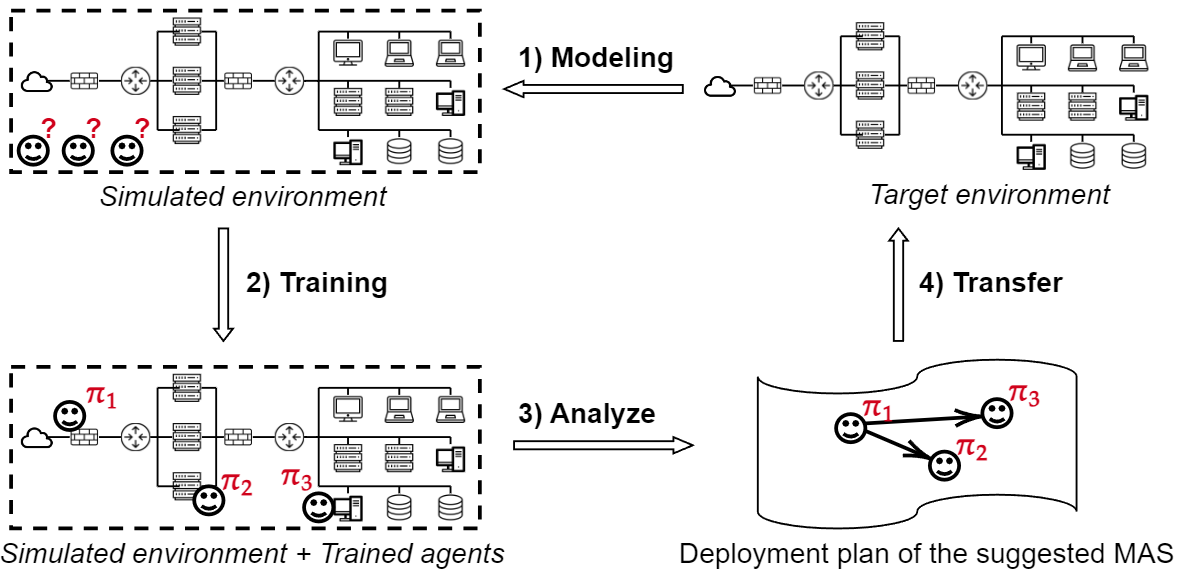
\includegraphics[width=1.2\linewidth]{figures/mamad_framework.png}
        \caption{Cycle de vie d'un SMA conçu avec MAMAD}
        \label{fig:cycle}
      \end{figure}
    \end{column}
  \end{columns}

\end{frame}

\begin{frame}{Modélisation en simulation}{Cadre}

  \textbf{Un environnement en réseau}
  \begin{itemize}
    \item Propriétés : ouvert, dynamique/statique, déterministe, accessible/inaccessible\dots
          \phantom{XXXXXXXXXXXXXXXXXXXXXXXXXXXXXXXXXXXXXXXXXXXXXXXXXXXXXXXXXXXXXXXX}
  \end{itemize}

  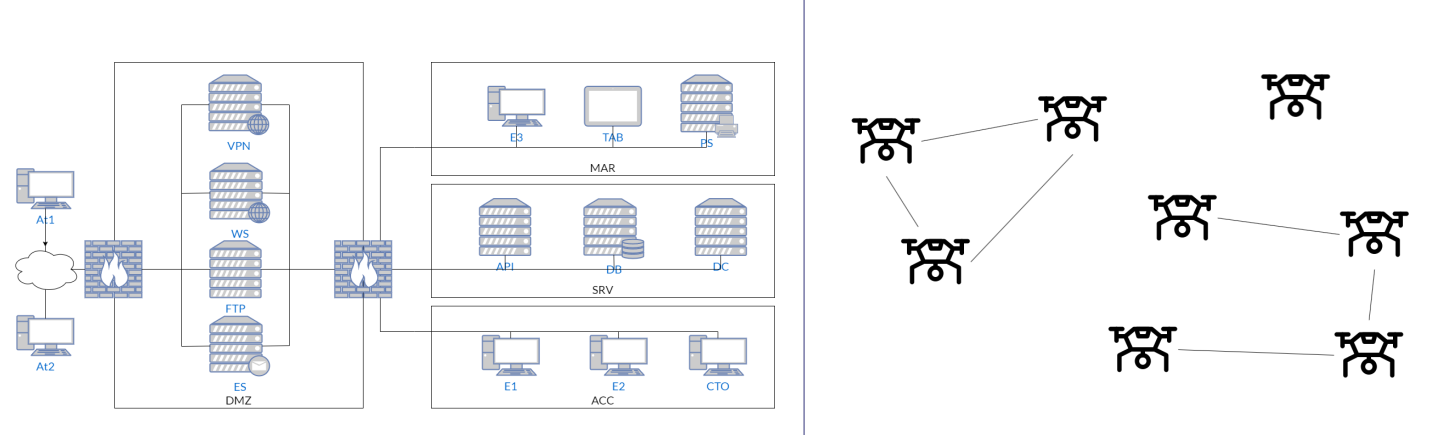
\includegraphics[width=\linewidth, trim=0cm 0cm 0cm 0.1cm, clip]{figures/0.png}

\end{frame}

\begin{frame}{Modélisation en simulation}{Cadre}

  \textbf{Avec une Green Team}
  \begin{itemize}
    \item Utilisateurs \textquote{normaux} : sessions, requêtes, scan des ports, envoi de données
          \phantom{XXXXXXXXXXXXXXXXXXXXXXXXXXXXXXXXXXXXXXXXXXXXXXXXXXXXXXXXXXXXXXXX}
  \end{itemize}

  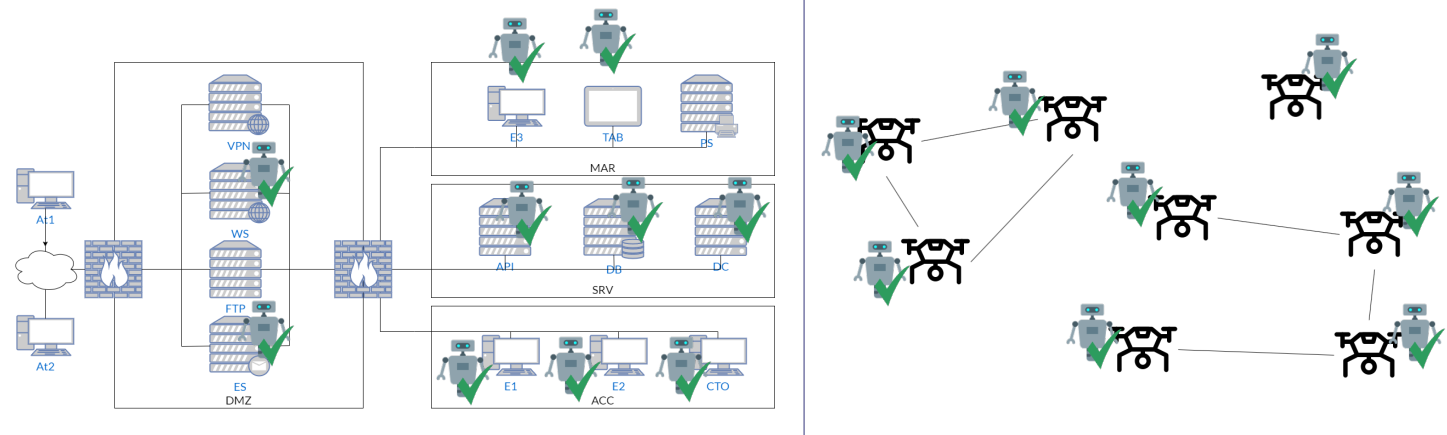
\includegraphics[width=\linewidth, trim=0cm 0cm 0cm 0.1cm, clip]{figures/1.png}
\end{frame}

\begin{frame}{Modélisation en simulation}{Cadre}

  \textbf{Avec une Red Team}
  \begin{itemize}
    \item Cyber-attaquants : découverte de nœuds/services, exploitation des vulnérabilités, escalade de privilège, déplacement latéral, impact\dots
  \end{itemize}

  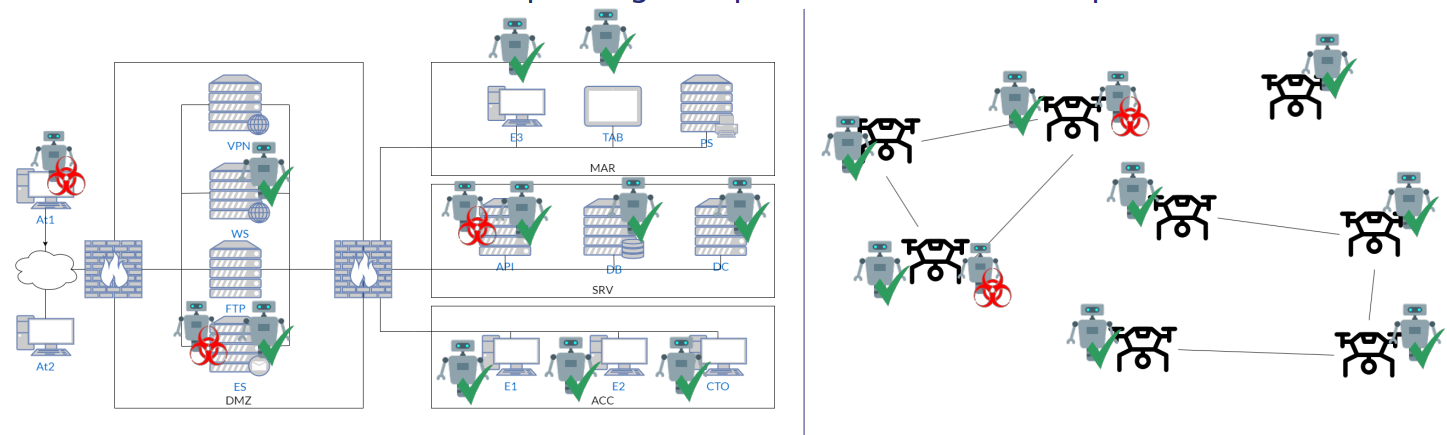
\includegraphics[width=\linewidth, trim=0cm 0cm 0cm 0.1cm, clip]{figures/2.png}
\end{frame}

\begin{frame}{Modélisation en simulation}{Cadre}

  \textbf{Avec une Blue Team}
  \begin{itemize}
    \item Cyber-défenseurs : analyse de menace, contrôle des accès, tuer des processus suspects, mise en place de \textquote{honey pots}, re-imager un nœud\dots
  \end{itemize}

  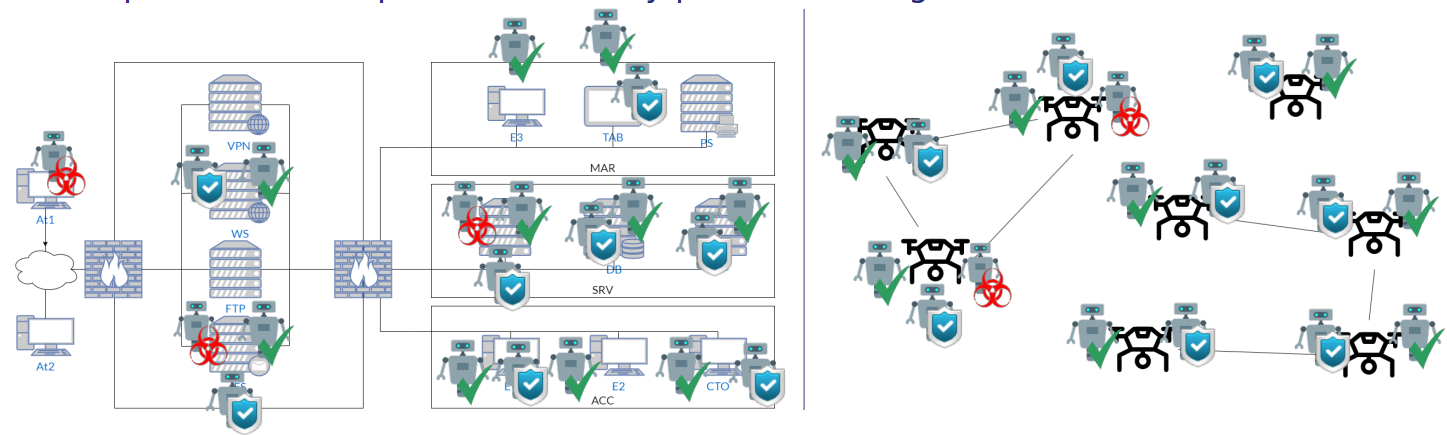
\includegraphics[width=\linewidth, trim=0cm 0cm 0cm 0.1cm, clip]{figures/3.png}
\end{frame}

\begin{frame}{Modélisation en simulation}{Modèle Markovien}

  \begin{columns}[c]

    \hspace{-1.cm}

    \begin{column}{0.5\textwidth}

      \begin{itemize}
        \item Modèle Markovien (Dec-POMDP)
              \begin{itemize}
                \item Prise de décision collective
                \item Modélisation de incertitude des actions / observations
                \item \textbf{T : Fonction transition état}
              \end{itemize}

        \item[\phantom{X}] \phantom{Modélisation manuelle de T}
          \begin{itemize}
            \item[\phantom{X}] \phantom{CybORG}
          \end{itemize}
        \item[\phantom{X}] \phantom{Modélisation automatisée de T}
          \begin{enumerate}
            \item[\phantom{X}] \phantom{Collecte traces réelles}
            \item[\phantom{X}] \phantom{Entrainement via un RNN (LSTM)}
          \end{enumerate}
      \end{itemize}

    \end{column}

    \hspace{-1.5cm}

    \begin{column}{0.6\textwidth}
      \centering
      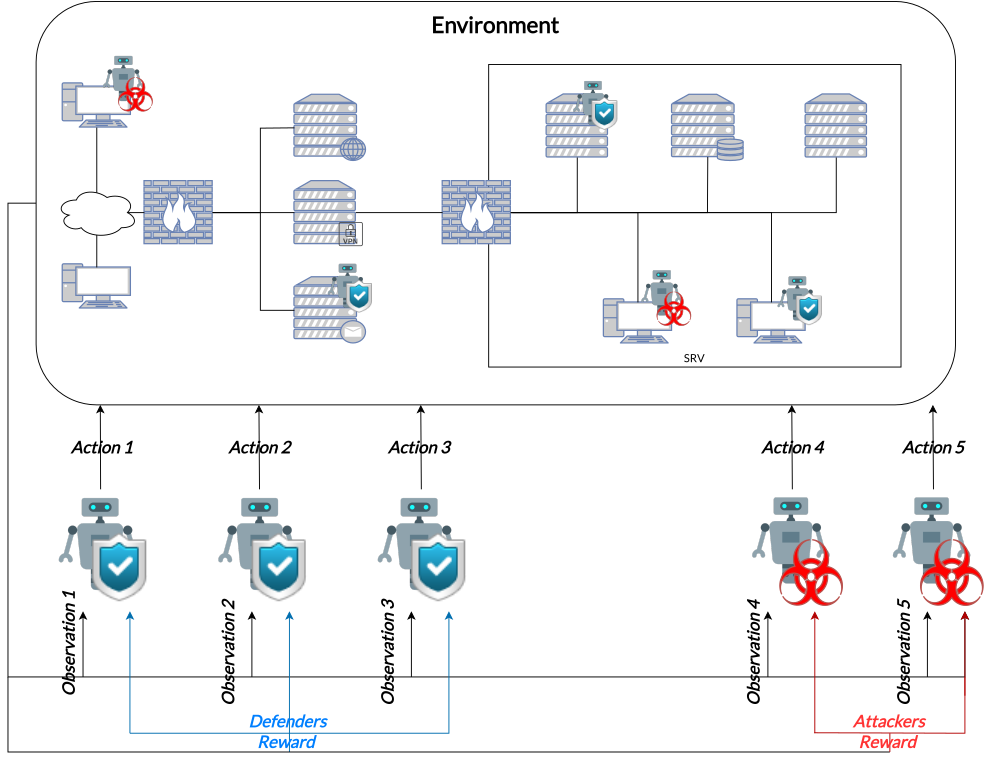
\includegraphics[width=\linewidth]{figures/marl_framework.png}
    \end{column}
  \end{columns}

  \medskip

  {\tiny \begin{spacing}{0.8}
      \textit{Soulé, J., Jamont, J.-P., Occello, M., Théron, P., \& Traonouez, L.-M. Towards a Multi-Agent Simulation of Cyber-attackers and Cyber-defenders Battles. IEEE SMC 2023.}
    \end{spacing}}

\end{frame}


\begin{frame}{Modélisation en simulation}{Modèle Markovien}

  \begin{columns}[c]

    \hspace{-1.cm}

    \begin{column}{0.5\textwidth}

      \begin{itemize}
        \item Modèle Markovien (Dec-POMDP)
              \begin{itemize}
                \item Prise de décision collective
                \item Modélisation de incertitude des actions / observations
                \item \textbf{T : Fonction transition état}
              \end{itemize}

        \item Modélisation manuelle de T
              \begin{itemize}
                \item CybORG
              \end{itemize}
        \item[\phantom{X}] \phantom{Modélisation automatisée de T}
          \begin{enumerate}
            \item[\phantom{X}] \phantom{Collecte traces réelles}
            \item[\phantom{X}] \phantom{Entrainement via un RNN (LSTM)}
          \end{enumerate}
      \end{itemize}

    \end{column}

    \hspace{-1.5cm}

    \begin{column}{0.6\textwidth}
      \centering
      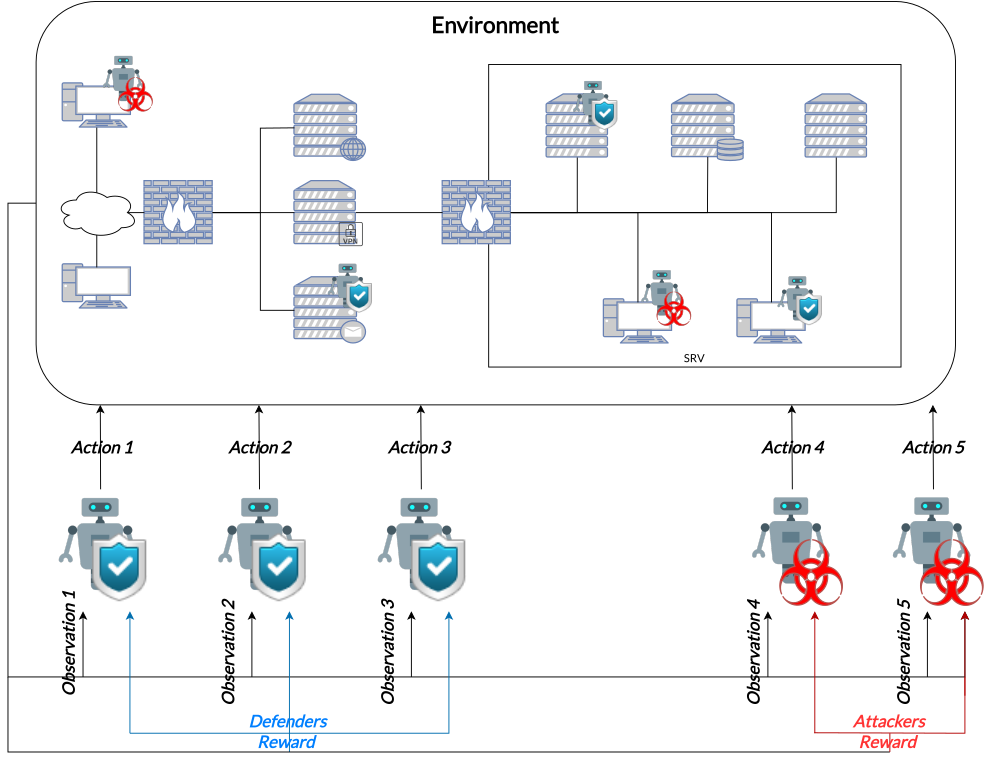
\includegraphics[width=\linewidth]{figures/marl_framework.png}
    \end{column}
  \end{columns}

  \medskip

  {\tiny \begin{spacing}{0.8}
      \textit{Soulé, J., Jamont, J.-P., Occello, M., Théron, P., \& Traonouez, L.-M. Towards a Multi-Agent Simulation of Cyber-attackers and Cyber-defenders Battles. IEEE SMC 2023.}
    \end{spacing}}

\end{frame}


\begin{frame}{Modélisation en simulation}{Modèle Markovien}

  \begin{columns}[c]

    \hspace{-1.cm}

    \begin{column}{0.5\textwidth}

      \begin{itemize}
        \item Modèle Markovien (Dec-POMDP)
              \begin{itemize}
                \item Prise de décision collective
                \item Modélisation de incertitude des actions / observations
                \item \textbf{T : Fonction transition état}
              \end{itemize}

        \item Modélisation manuelle de T
              \begin{itemize}
                \item CybORG
              \end{itemize}
        \item Modélisation automatisée de T
              \begin{enumerate}
                \item Collecte traces réelles
                \item Entrainement via un RNN (LSTM)
              \end{enumerate}
      \end{itemize}

    \end{column}

    \hspace{-1.5cm}

    \begin{column}{0.6\textwidth}
      \centering
      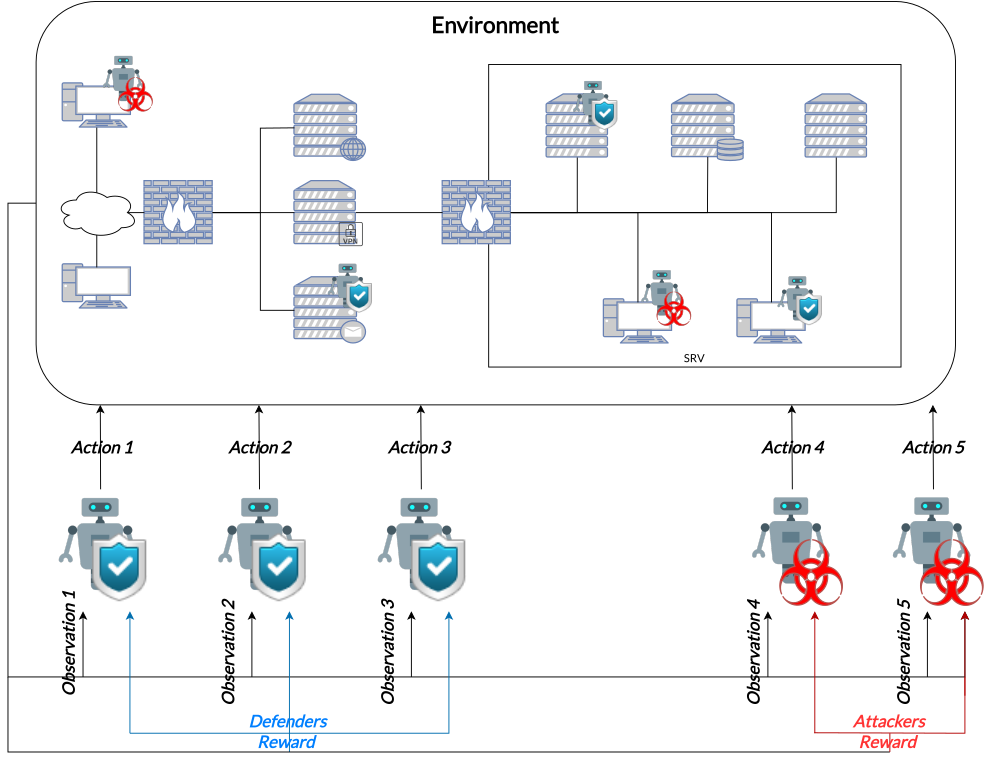
\includegraphics[width=\linewidth]{figures/marl_framework.png}
    \end{column}
  \end{columns}

  \medskip

  {\tiny \begin{spacing}{0.8}
      \textit{Soulé, J., Jamont, J.-P., Occello, M., Théron, P., \& Traonouez, L.-M. Towards a Multi-Agent Simulation of Cyber-attackers and Cyber-defenders Battles. IEEE SMC 2023.}
    \end{spacing}}

\end{frame}



\begin{frame}{Apprentissage guidé/contraint}

  \textbf{MARL \textquote{Vanilla}}
  \begin{itemize}
    \item Choisir les meilleures actions pour maximiser récompense cumulée
  \end{itemize}

  \begin{center}
    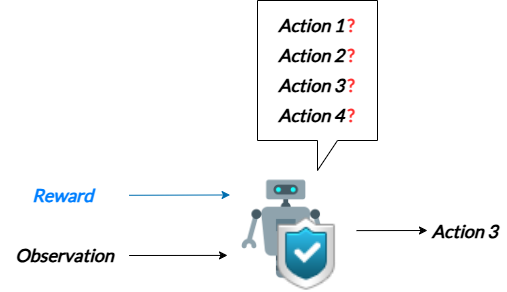
\includegraphics[width=0.5\linewidth]{figures/vanilla_marl.png}
  \end{center}

  \vfill

  {\tiny \begin{spacing}{0.8}
      \textit{Soulé, J., Jamont, J.-P., Occello, M., Traonouez, L.-M., \& Théron, P. An Organizationally-Oriented Approach to Enhancing Explainability and Control in Multi-Agent Reinforcement Learning. Proceedings of the 24th International Conference on Autonomous Agents and Multiagent Systems (AAMAS 2025), Detroit, Michigan, USA, 2025.}
    \end{spacing}}

\end{frame}

\begin{frame}{Apprentissage guidé/contraint}

  \textbf{MARL + Organisation ($\mathcal{M}OISE^+$)}
  \begin{itemize}
    \item Rôle : imposer/refuser actions $\rightarrow$ garantie de sûreté
  \end{itemize}

  \begin{center}
    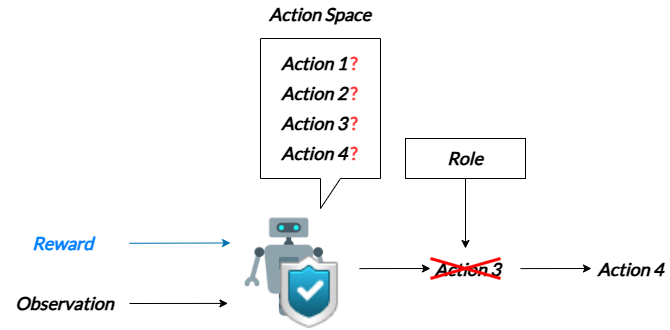
\includegraphics[width=0.5\linewidth]{figures/role_marl.png}
  \end{center}

  \vfill

  {\tiny \begin{spacing}{0.8}
      \textit{Soulé, J., Jamont, J.-P., Occello, M., Traonouez, L.-M., \& Théron, P. An Organizationally-Oriented Approach to Enhancing Explainability and Control in Multi-Agent Reinforcement Learning. Proceedings of the 24th International Conference on Autonomous Agents and Multiagent Systems (AAMAS 2025), Detroit, Michigan, USA, 2025.}
    \end{spacing}}

\end{frame}

\begin{frame}{Apprentissage guidé/contraint}

  \textbf{MARL + Organisation ($\mathcal{M}OISE^+$)}
  \begin{itemize}
    \item Objectif : inciter à atteindre un objectif intermédiaire
  \end{itemize}

  \begin{center}
    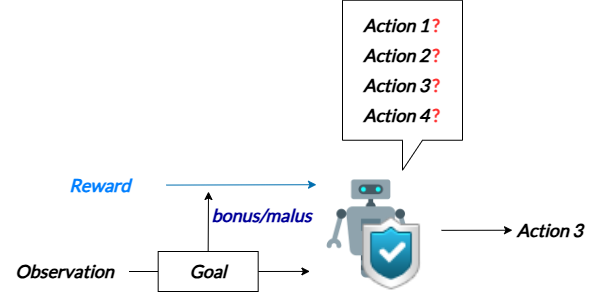
\includegraphics[width=0.5\linewidth]{figures/goal_marl.png}
  \end{center}

  \vfill

  {\tiny \begin{spacing}{0.8}
      \textit{Soulé, J., Jamont, J.-P., Occello, M., Traonouez, L.-M., \& Théron, P. An Organizationally-Oriented Approach to Enhancing Explainability and Control in Multi-Agent Reinforcement Learning. Proceedings of the 24th International Conference on Autonomous Agents and Multiagent Systems (AAMAS 2025), Detroit, Michigan, USA, 2025.}
    \end{spacing}}

\end{frame}


\begin{frame}{Analyse post-entrainement}

  \textbf{Trajectory-based Evaluation in MOISE+MARL (TEMM)}
  \begin{itemize}
    \item \textbf{Objectif} : Fournir une interprétation a posteriori du comportement des agents à un niveau organisationnel.
  \end{itemize}

  \vspace{1em}
  \textbf{Hypothèses sous-jacentes :}
  \begin{itemize}
    \item \textbf{Rôles} $\sim$ motifs fréquents de transitions \emph{(observation, action)} dans les trajectoires des agents.
    \item \textbf{Objectifs} $\sim$ observations reçues fréquemment au sein des trajectoires des agents.
  \end{itemize}

  \vspace{0.8cm}
  \begin{center}
    \begin{columns}[c]

      \begin{column}{0.4\textwidth}
        \centering
        


\tikzset{every picture/.style={line width=0.75pt}} %set default line width to 0.75pt        

\begin{tikzpicture}[x=0.75pt,y=0.75pt,yscale=-1,xscale=1]
%uncomment if require: \path (0,1974); %set diagram left start at 0, and has height of 1974

%Shape: Rectangle [id:dp9996076613305621] 
\draw  [fill={rgb, 255:red, 255; green, 255; blue, 255 }  ,fill opacity=1 ] (24,1558.11) -- (176.1,1558.11) -- (176.1,1644) -- (24,1644) -- cycle ;
%Straight Lines [id:da05824332013205091] 
\draw [color={rgb, 255:red, 208; green, 2; blue, 27 }  ,draw opacity=1 ]   (142.67,1570.84) -- (124.28,1577.49) -- (87.26,1592.41) -- (108.68,1604.12) -- (93.53,1601.36) -- (86.58,1603.01) -- (86.58,1612.77) -- (82.05,1616.07) -- (81.22,1616.67) -- (78.65,1614.8) -- (70.51,1608.86) -- (54.44,1608.86) -- (57,1610.73) -- (49.09,1612.77) -- (51.85,1616.79) -- (38.38,1628.38) ;
\draw [shift={(145.49,1569.82)}, rotate = 160.12] [fill={rgb, 255:red, 208; green, 2; blue, 27 }  ,fill opacity=1 ][line width=0.08]  [draw opacity=0] (3.57,-1.72) -- (0,0) -- (3.57,1.72) -- cycle    ;
%Straight Lines [id:da9249559779542824] 
\draw [color={rgb, 255:red, 80; green, 227; blue, 194 }  ,draw opacity=1 ]   (143.47,1568.13) -- (134.78,1577.63) -- (113.36,1577.63) -- (113.36,1585.44) -- (86.58,1593.25) -- (91.93,1597.15) -- (97.29,1604.96) -- (81.22,1601.06) -- (86.58,1608.86) -- (81.22,1608.86) -- (86.58,1616.67) -- (75.87,1616.67) -- (67.94,1608.94) -- (65.16,1614.72) -- (43.73,1603.01) -- (59.8,1616.67) -- (43.73,1608.86) -- (49.09,1616.67) -- (43.73,1632.29) ;
\draw [shift={(145.49,1565.92)}, rotate = 132.45] [fill={rgb, 255:red, 80; green, 227; blue, 194 }  ,fill opacity=1 ][line width=0.08]  [draw opacity=0] (3.57,-1.72) -- (0,0) -- (3.57,1.72) -- cycle    ;
%Straight Lines [id:da17118391857757054] 
\draw [color={rgb, 255:red, 248; green, 231; blue, 28 }  ,draw opacity=1 ]   (153.23,1574.14) -- (126.83,1577.75) -- (124.07,1581.54) -- (105.41,1585.56) -- (91.93,1593.25) -- (93.53,1601.36) -- (89.34,1605.08) -- (81.22,1597.15) -- (91.93,1612.77) -- (91.93,1616.67) -- (81.22,1616.67) -- (59.99,1609.06) -- (57.21,1614.84) -- (41.14,1616.79) -- (35.78,1632.41) ;
\draw [shift={(156.2,1573.73)}, rotate = 172.2] [fill={rgb, 255:red, 248; green, 231; blue, 28 }  ,fill opacity=1 ][line width=0.08]  [draw opacity=0] (3.57,-1.72) -- (0,0) -- (3.57,1.72) -- cycle    ;
%Straight Lines [id:da6427777277243145] 
\draw [color={rgb, 255:red, 144; green, 19; blue, 254 }  ,draw opacity=1 ]   (160.23,1577.39) -- (165.84,1578.41) -- (161.56,1573.73) -- (157.27,1570.61) -- (164.86,1573.73) -- (170.13,1578.41) -- (161.56,1583.1) -- (166.91,1589.34) -- (161.56,1597.15) -- (166.91,1601.06) -- (161.56,1612.77) -- (161.56,1628.38) -- (145.49,1624.48) -- (134.78,1624.48) -- (128.99,1623.07) -- (125.92,1622.33) -- (121.57,1621.27) -- (118.71,1620.58) -- (107.96,1619.71) -- (99.43,1619.01) -- (95.23,1618.25) -- (86.58,1616.67) -- (75.87,1616.67) -- (70.51,1620.58) -- (59.8,1624.48) -- (59.8,1632.29) ;
\draw [shift={(157.27,1576.85)}, rotate = 10.33] [fill={rgb, 255:red, 144; green, 19; blue, 254 }  ,fill opacity=1 ][line width=0.08]  [draw opacity=0] (3.57,-1.72) -- (0,0) -- (3.57,1.72) -- cycle    ;
%Straight Lines [id:da7390021320622445] 
\draw [color={rgb, 255:red, 65; green, 117; blue, 5 }  ,draw opacity=1 ]   (159.15,1578.17) -- (164.77,1579.19) -- (160.49,1574.51) -- (156.2,1571.39) -- (163.79,1574.51) -- (169.06,1579.19) -- (161.56,1587.78) -- (165.84,1590.13) -- (163.7,1601.84) -- (150.85,1597.15) -- (161.56,1603.4) -- (174.41,1615.89) -- (157.27,1606.52) -- (160.49,1613.55) -- (163.7,1625.26) -- (152.99,1628.38) -- (135.85,1622.14) -- (123,1622.14) -- (116.57,1622.14) -- (110.14,1620.58) -- (108,1623.7) -- (103.72,1620.58) -- (105.86,1625.26) -- (94.16,1619.03) -- (85.51,1617.45) -- (74.8,1617.45) -- (69.44,1621.36) -- (58.73,1625.26) -- (58.73,1633.07) ;
\draw [shift={(156.2,1577.63)}, rotate = 10.33] [fill={rgb, 255:red, 65; green, 117; blue, 5 }  ,fill opacity=1 ][line width=0.08]  [draw opacity=0] (3.57,-1.72) -- (0,0) -- (3.57,1.72) -- cycle    ;
%Shape: Ellipse [id:dp30050508180239144] 
\draw  [draw opacity=0][fill={rgb, 255:red, 208; green, 2; blue, 27 }  ,fill opacity=0.62 ] (46.49,1615.89) .. controls (46.49,1614.6) and (47.93,1613.55) .. (49.71,1613.55) .. controls (51.48,1613.55) and (52.92,1614.6) .. (52.92,1615.89) .. controls (52.92,1617.19) and (51.48,1618.23) .. (49.71,1618.23) .. controls (47.93,1618.23) and (46.49,1617.19) .. (46.49,1615.89) -- cycle ;
%Shape: Ellipse [id:dp15311501498248647] 
\draw  [draw opacity=0][fill={rgb, 255:red, 208; green, 2; blue, 27 }  ,fill opacity=0.62 ] (90.49,1619.03) .. controls (90.49,1617.74) and (91.93,1616.69) .. (93.71,1616.69) .. controls (95.48,1616.69) and (96.92,1617.74) .. (96.92,1619.03) .. controls (96.92,1620.32) and (95.48,1621.37) .. (93.71,1621.37) .. controls (91.93,1621.37) and (90.49,1620.32) .. (90.49,1619.03) -- cycle ;
%Shape: Ellipse [id:dp19167487081496637] 
\draw  [draw opacity=0][fill={rgb, 255:red, 208; green, 2; blue, 27 }  ,fill opacity=0.62 ] (161.11,1606.52) .. controls (161.11,1605.23) and (162.54,1604.18) .. (164.32,1604.18) .. controls (166.09,1604.18) and (167.53,1605.23) .. (167.53,1606.52) .. controls (167.53,1607.82) and (166.09,1608.86) .. (164.32,1608.86) .. controls (162.54,1608.86) and (161.11,1607.82) .. (161.11,1606.52) -- cycle ;
%Shape: Ellipse [id:dp9201279867822619] 
\draw  [draw opacity=0][fill={rgb, 255:red, 208; green, 2; blue, 27 }  ,fill opacity=0.62 ] (120.4,1622.92) .. controls (120.4,1621.62) and (121.84,1620.58) .. (123.62,1620.58) .. controls (125.39,1620.58) and (126.83,1621.62) .. (126.83,1622.92) .. controls (126.83,1624.21) and (125.39,1625.26) .. (123.62,1625.26) .. controls (121.84,1625.26) and (120.4,1624.21) .. (120.4,1622.92) -- cycle ;
%Shape: Ellipse [id:dp3048334813609519] 
\draw  [draw opacity=0][fill={rgb, 255:red, 208; green, 2; blue, 27 }  ,fill opacity=0.62 ] (161.11,1590.91) .. controls (161.11,1589.61) and (162.54,1588.56) .. (164.32,1588.56) .. controls (166.09,1588.56) and (167.53,1589.61) .. (167.53,1590.91) .. controls (167.53,1592.2) and (166.09,1593.25) .. (164.32,1593.25) .. controls (162.54,1593.25) and (161.11,1592.2) .. (161.11,1590.91) -- cycle ;
%Shape: Ellipse [id:dp7290465976812913] 
\draw  [draw opacity=0][fill={rgb, 255:red, 208; green, 2; blue, 27 }  ,fill opacity=0.62 ] (86.13,1603.4) .. controls (86.13,1602.11) and (87.56,1601.06) .. (89.34,1601.06) .. controls (91.11,1601.06) and (92.55,1602.11) .. (92.55,1603.4) .. controls (92.55,1604.69) and (91.11,1605.74) .. (89.34,1605.74) .. controls (87.56,1605.74) and (86.13,1604.69) .. (86.13,1603.4) -- cycle ;
%Shape: Ellipse [id:dp6154487622646608] 
\draw  [draw opacity=0][fill={rgb, 255:red, 208; green, 2; blue, 27 }  ,fill opacity=0.62 ] (109.69,1583.1) .. controls (109.69,1581.8) and (111.13,1580.76) .. (112.9,1580.76) .. controls (114.68,1580.76) and (116.12,1581.8) .. (116.12,1583.1) .. controls (116.12,1584.39) and (114.68,1585.44) .. (112.9,1585.44) .. controls (111.13,1585.44) and (109.69,1584.39) .. (109.69,1583.1) -- cycle ;
%Shape: Ellipse [id:dp6108483574180856] 
\draw  [draw opacity=0][fill={rgb, 255:red, 189; green, 16; blue, 224 }  ,fill opacity=0.8 ] (77.56,1615.89) .. controls (77.56,1614.6) and (79,1613.55) .. (80.77,1613.55) .. controls (82.55,1613.55) and (83.98,1614.6) .. (83.98,1615.89) .. controls (83.98,1617.19) and (82.55,1618.23) .. (80.77,1618.23) .. controls (79,1618.23) and (77.56,1617.19) .. (77.56,1615.89) -- cycle ;
%Shape: Ellipse [id:dp08863924891219843] 
\draw  [draw opacity=0][fill={rgb, 255:red, 208; green, 2; blue, 27 }  ,fill opacity=0.62 ] (84.52,1609.06) .. controls (84.52,1607.77) and (85.96,1606.72) .. (87.73,1606.72) .. controls (89.51,1606.72) and (90.95,1607.77) .. (90.95,1609.06) .. controls (90.95,1610.35) and (89.51,1611.4) .. (87.73,1611.4) .. controls (85.96,1611.4) and (84.52,1610.35) .. (84.52,1609.06) -- cycle ;
%Shape: Ellipse [id:dp49807154634681794] 
\draw  [draw opacity=0][fill={rgb, 255:red, 208; green, 2; blue, 27 }  ,fill opacity=0.62 ] (91.21,1601.64) .. controls (91.21,1600.35) and (92.65,1599.3) .. (94.43,1599.3) .. controls (96.2,1599.3) and (97.64,1600.35) .. (97.64,1601.64) .. controls (97.64,1602.94) and (96.2,1603.98) .. (94.43,1603.98) .. controls (92.65,1603.98) and (91.21,1602.94) .. (91.21,1601.64) -- cycle ;
%Shape: Ellipse [id:dp17062416794692736] 
\draw  [draw opacity=0][fill={rgb, 255:red, 208; green, 2; blue, 27 }  ,fill opacity=0.62 ] (100.59,1619.41) .. controls (100.59,1618.11) and (102.03,1617.06) .. (103.8,1617.06) .. controls (105.57,1617.06) and (107.01,1618.11) .. (107.01,1619.41) .. controls (107.01,1620.7) and (105.57,1621.75) .. (103.8,1621.75) .. controls (102.03,1621.75) and (100.59,1620.7) .. (100.59,1619.41) -- cycle ;
%Shape: Ellipse [id:dp05427293190477478] 
\draw  [draw opacity=0][fill={rgb, 255:red, 189; green, 16; blue, 224 }  ,fill opacity=0.8 ] (152.54,1626.82) .. controls (152.54,1625.53) and (153.98,1624.48) .. (155.75,1624.48) .. controls (157.52,1624.48) and (158.96,1625.53) .. (158.96,1626.82) .. controls (158.96,1628.12) and (157.52,1629.16) .. (155.75,1629.16) .. controls (153.98,1629.16) and (152.54,1628.12) .. (152.54,1626.82) -- cycle ;
%Shape: Ellipse [id:dp0565658994925915] 
\draw  [draw opacity=0][fill={rgb, 255:red, 208; green, 2; blue, 27 }  ,fill opacity=0.62 ] (158.96,1616.67) .. controls (158.96,1615.38) and (160.4,1614.33) .. (162.18,1614.33) .. controls (163.95,1614.33) and (165.39,1615.38) .. (165.39,1616.67) .. controls (165.39,1617.97) and (163.95,1619.01) .. (162.18,1619.01) .. controls (160.4,1619.01) and (158.96,1617.97) .. (158.96,1616.67) -- cycle ;
%Shape: Ellipse [id:dp5007110255270828] 
\draw  [draw opacity=0][fill={rgb, 255:red, 189; green, 16; blue, 224 }  ,fill opacity=0.8 ] (57,1610.73) .. controls (57,1609.43) and (58.44,1608.38) .. (60.21,1608.38) .. controls (61.99,1608.38) and (63.43,1609.43) .. (63.43,1610.73) .. controls (63.43,1612.02) and (61.99,1613.07) .. (60.21,1613.07) .. controls (58.44,1613.07) and (57,1612.02) .. (57,1610.73) -- cycle ;
%Shape: Ellipse [id:dp22598728144573377] 
\draw  [draw opacity=0][fill={rgb, 255:red, 208; green, 2; blue, 27 }  ,fill opacity=0.62 ] (88.72,1595.59) .. controls (88.72,1594.3) and (90.16,1593.25) .. (91.93,1593.25) .. controls (93.71,1593.25) and (95.15,1594.3) .. (95.15,1595.59) .. controls (95.15,1596.88) and (93.71,1597.93) .. (91.93,1597.93) .. controls (90.16,1597.93) and (88.72,1596.88) .. (88.72,1595.59) -- cycle ;
%Shape: Ellipse [id:dp14749486568088088] 
\draw  [draw opacity=0][fill={rgb, 255:red, 189; green, 16; blue, 224 }  ,fill opacity=0.8 ] (93.54,1589.34) .. controls (93.54,1588.05) and (94.98,1587) .. (96.75,1587) .. controls (98.53,1587) and (99.97,1588.05) .. (99.97,1589.34) .. controls (99.97,1590.64) and (98.53,1591.69) .. (96.75,1591.69) .. controls (94.98,1591.69) and (93.54,1590.64) .. (93.54,1589.34) -- cycle ;
%Shape: Polygon Curved [id:ds6643267525526769] 
\draw  [color={rgb, 255:red, 74; green, 144; blue, 226 }  ,draw opacity=1 ][fill={rgb, 255:red, 74; green, 144; blue, 226 }  ,fill opacity=0.5 ] (27.21,1628.38) .. controls (30.38,1623.39) and (36.63,1621.99) .. (42.56,1622.18) .. controls (47.05,1622.33) and (51.36,1623.39) .. (53.99,1624.48) .. controls (60.1,1627.02) and (65.56,1626.63) .. (64.7,1632.29) .. controls (63.85,1637.95) and (56.88,1637.17) .. (48.64,1636.19) .. controls (40.39,1635.22) and (21.64,1637.17) .. (27.21,1628.38) -- cycle ;
%Shape: Polygon Curved [id:ds9461514343962948] 
\draw  [color={rgb, 255:red, 208; green, 2; blue, 27 }  ,draw opacity=1 ][fill={rgb, 255:red, 208; green, 2; blue, 27 }  ,fill opacity=0.5 ] (139.68,1569.82) .. controls (145.25,1561.04) and (148.01,1561.59) .. (145.04,1565.92) .. controls (142.07,1570.25) and (154.68,1563.87) .. (153.82,1569.53) .. controls (152.97,1575.19) and (169.35,1578.61) .. (161.11,1577.63) .. controls (152.86,1576.66) and (134.11,1578.61) .. (139.68,1569.82) -- cycle ;
%Shape: Ellipse [id:dp06406072166611776] 
\draw  [draw opacity=0][fill={rgb, 255:red, 208; green, 2; blue, 27 }  ,fill opacity=0.62 ] (71.13,1617.45) .. controls (71.13,1616.16) and (72.57,1615.11) .. (74.34,1615.11) .. controls (76.12,1615.11) and (77.56,1616.16) .. (77.56,1617.45) .. controls (77.56,1618.75) and (76.12,1619.8) .. (74.34,1619.8) .. controls (72.57,1619.8) and (71.13,1618.75) .. (71.13,1617.45) -- cycle ;
%Shape: Ellipse [id:dp049221150011381054] 
\draw  [draw opacity=0][fill={rgb, 255:red, 189; green, 16; blue, 224 }  ,fill opacity=0.8 ] (56.59,1624.48) .. controls (56.59,1623.19) and (58.03,1622.14) .. (59.8,1622.14) .. controls (61.58,1622.14) and (63.01,1623.19) .. (63.01,1624.48) .. controls (63.01,1625.77) and (61.58,1626.82) .. (59.8,1626.82) .. controls (58.03,1626.82) and (56.59,1625.77) .. (56.59,1624.48) -- cycle ;


% Text Node
\draw (68.95,1583.75) node  [font=\tiny,color={rgb, 255:red, 189; green, 16; blue, 224 }  ,opacity=1 ] [align=left] {$\displaystyle g_{5} =\{\omega _{21} \dotsc \}$};
% Text Node
\draw (82.63,1627.35) node  [font=\tiny,color={rgb, 255:red, 189; green, 16; blue, 224 }  ,opacity=1 ] [align=left] {$\displaystyle g_{2} =\{\omega _{5}\}$};
% Text Node
\draw (152.91,1586.86) node  [font=\tiny,color={rgb, 255:red, 189; green, 16; blue, 224 }  ,opacity=1 ] [align=left] {$\displaystyle ...$};
% Text Node
\draw (101.5,1575.93) node  [font=\tiny,color={rgb, 255:red, 189; green, 16; blue, 224 }  ,opacity=1 ] [align=left] {$\displaystyle ...$};
% Text Node
\draw (136.45,1636.35) node  [font=\tiny,color={rgb, 255:red, 189; green, 16; blue, 224 }  ,opacity=1 ] [align=left] {$\displaystyle g_{4} =\{\omega _{301} ,\omega _{302}\}$};
% Text Node
\draw (113.58,1612.35) node  [font=\tiny,color={rgb, 255:red, 189; green, 16; blue, 224 }  ,opacity=1 ] [align=left] {$\displaystyle g_{3} =\{\omega _{10}\}$};
% Text Node
\draw (55.11,1600.35) node  [font=\tiny,color={rgb, 255:red, 189; green, 16; blue, 224 }  ,opacity=1 ] [align=left] {$\displaystyle g_{1} =\{\omega _{1}\}$};
% Text Node
\draw (105.58,1568.35) node  [font=\tiny,color={rgb, 255:red, 202; green, 52; blue, 69 }  ,opacity=1 ] [align=left] {$\displaystyle g_{*} =\Omega _{goal}$};
% Text Node
\draw (73.43,1637.35) node  [font=\tiny,color={rgb, 255:red, 74; green, 144; blue, 226 }  ,opacity=1 ] [align=left] {$\displaystyle \Omega _{init}$};
% Text Node
\draw (32.91,1567.84) node  [font=\scriptsize] [align=left] {$\displaystyle \Omega $};
% Text Node
\draw (93.61,1653) node   [align=left] {{\tiny \textit{An abstract visualization of}}};
\draw (93.61,1662) node   [align=left] {{\tiny \textit{observations in trajectories}}};

\end{tikzpicture}
      \end{column}

      \begin{column}{0.1\textwidth}
      \end{column}

      \begin{column}{0.4\textwidth}
        \centering
        


\tikzset{every picture/.style={line width=0.75pt}} %set default line width to 0.75pt        

\begin{tikzpicture}[x=0.75pt,y=0.75pt,yscale=-1,xscale=1]
%uncomment if require: \path (0,1974); %set diagram left start at 0, and has height of 1974

%Shape: Rectangle [id:dp5335676631264512] 
\draw  [fill={rgb, 255:red, 255; green, 255; blue, 255 }  ,fill opacity=1 ] (190,1560.11) -- (342.1,1560.11) -- (342.1,1646) -- (190,1646) -- cycle ;
%Straight Lines [id:da6623576988919416] 
\draw [color={rgb, 255:red, 208; green, 2; blue, 27 }  ,draw opacity=1 ]   (308.67,1572.84) -- (290.28,1579.49) -- (253.26,1594.41) -- (292.1,1604) -- (274.1,1612) -- (262.1,1616) -- (252.58,1614.77) -- (246.1,1604) -- (240.1,1604) -- (236.1,1606) -- (236.51,1610.86) -- (220.44,1610.86) -- (223,1612.73) -- (215.09,1614.77) -- (217.85,1618.79) -- (204.38,1630.38) ;
\draw [shift={(311.49,1571.82)}, rotate = 160.12] [fill={rgb, 255:red, 208; green, 2; blue, 27 }  ,fill opacity=1 ][line width=0.08]  [draw opacity=0] (3.57,-1.72) -- (0,0) -- (3.57,1.72) -- cycle    ;
%Straight Lines [id:da5424854363807742] 
\draw [color={rgb, 255:red, 80; green, 227; blue, 194 }  ,draw opacity=1 ]   (309.47,1570.13) -- (300.78,1579.63) -- (279.36,1579.63) -- (279.36,1587.44) -- (252.58,1595.25) -- (250.1,1598) -- (248.1,1600) -- (247.22,1603.06) -- (252.58,1610.86) -- (247.22,1610.86) -- (242.1,1608) -- (242.1,1610) -- (233.94,1610.94) -- (231.16,1616.72) -- (209.73,1605.01) -- (225.8,1618.67) -- (209.73,1610.86) -- (215.09,1618.67) -- (209.73,1634.29) ;
\draw [shift={(311.49,1567.92)}, rotate = 132.45] [fill={rgb, 255:red, 80; green, 227; blue, 194 }  ,fill opacity=1 ][line width=0.08]  [draw opacity=0] (3.57,-1.72) -- (0,0) -- (3.57,1.72) -- cycle    ;
%Straight Lines [id:da21186841526109945] 
\draw [color={rgb, 255:red, 248; green, 231; blue, 28 }  ,draw opacity=1 ]   (319.23,1576.14) -- (292.83,1579.75) -- (290.07,1583.54) -- (271.41,1587.56) -- (257.93,1595.25) -- (280.1,1592) -- (284.1,1594) -- (290.1,1604) -- (257.93,1614.77) -- (257.93,1618.67) -- (247.22,1618.67) -- (225.99,1611.06) -- (223.21,1616.84) -- (207.14,1618.79) -- (201.78,1634.41) ;
\draw [shift={(322.2,1575.73)}, rotate = 172.2] [fill={rgb, 255:red, 248; green, 231; blue, 28 }  ,fill opacity=1 ][line width=0.08]  [draw opacity=0] (3.57,-1.72) -- (0,0) -- (3.57,1.72) -- cycle    ;
%Straight Lines [id:da6313290732282947] 
\draw [color={rgb, 255:red, 144; green, 19; blue, 254 }  ,draw opacity=1 ]   (326.23,1579.39) -- (331.84,1580.41) -- (327.56,1575.73) -- (323.27,1572.61) -- (330.86,1575.73) -- (336.13,1580.41) -- (327.56,1585.1) -- (332.91,1591.34) -- (324.1,1600) -- (330.1,1606) -- (312.1,1636) -- (320.1,1638) -- (306.1,1644) -- (306.1,1606) -- (300.1,1614) -- (311.49,1626.48) -- (300.78,1626.48) -- (294.99,1625.07) -- (291.92,1624.33) -- (287.57,1623.27) -- (284.71,1622.58) -- (273.96,1621.71) -- (265.43,1621.01) -- (261.23,1620.25) -- (250.1,1622) -- (241.87,1618.67) -- (236.51,1622.58) -- (225.8,1626.48) -- (225.8,1634.29) ;
\draw [shift={(323.27,1578.85)}, rotate = 10.33] [fill={rgb, 255:red, 144; green, 19; blue, 254 }  ,fill opacity=1 ][line width=0.08]  [draw opacity=0] (3.57,-1.72) -- (0,0) -- (3.57,1.72) -- cycle    ;
%Straight Lines [id:da1305524961942589] 
\draw [color={rgb, 255:red, 65; green, 117; blue, 5 }  ,draw opacity=1 ]   (325.15,1580.17) -- (330.77,1581.19) -- (326.49,1576.51) -- (322.2,1573.39) -- (329.79,1576.51) -- (335.06,1581.19) -- (327.56,1589.78) -- (331.84,1592.13) -- (329.7,1603.84) -- (316.85,1599.15) -- (327.56,1605.4) -- (314.1,1636) -- (318.1,1640) -- (310.1,1642) -- (304.1,1608) -- (298.1,1612) -- (301.85,1624.14) -- (289,1624.14) -- (282.57,1624.14) -- (276.14,1622.58) -- (274,1625.7) -- (269.72,1622.58) -- (271.86,1627.26) -- (260.16,1621.03) -- (251.51,1619.45) -- (240.8,1619.45) -- (235.44,1623.36) -- (224.73,1627.26) -- (224.73,1635.07) ;
\draw [shift={(322.2,1579.63)}, rotate = 10.33] [fill={rgb, 255:red, 65; green, 117; blue, 5 }  ,fill opacity=1 ][line width=0.08]  [draw opacity=0] (3.57,-1.72) -- (0,0) -- (3.57,1.72) -- cycle    ;
%Shape: Polygon Curved [id:ds29559681347985167] 
\draw  [color={rgb, 255:red, 184; green, 233; blue, 134 }  ,draw opacity=0 ][fill={rgb, 255:red, 74; green, 144; blue, 226 }  ,fill opacity=0.75 ] (203.31,1627.26) .. controls (208.88,1618.48) and (203.46,1612.19) .. (210,1608) .. controls (216.54,1603.81) and (229.5,1600.53) .. (248,1604) .. controls (266.5,1607.47) and (269.83,1605.44) .. (280,1604) .. controls (290.17,1602.56) and (250.44,1601.87) .. (252,1594) .. controls (253.56,1586.13) and (258.5,1591.77) .. (262,1588) .. controls (265.5,1584.23) and (314.2,1570.33) .. (316,1570) .. controls (317.8,1569.67) and (320.91,1572.43) .. (314,1576) .. controls (307.09,1579.57) and (294.2,1581.95) .. (288,1584) .. controls (281.8,1586.05) and (277.13,1589.32) .. (276,1590) .. controls (274.87,1590.68) and (280.1,1589.85) .. (284,1592) .. controls (287.9,1594.15) and (295.82,1601.53) .. (296,1602) .. controls (296.18,1602.47) and (264.78,1615.69) .. (264,1616) .. controls (263.22,1616.31) and (249.54,1612.38) .. (244,1612) .. controls (238.46,1611.62) and (217.32,1621.29) .. (214,1626) .. controls (210.68,1630.71) and (210.87,1632.35) .. (210,1636) .. controls (209.13,1639.65) and (197.74,1636.04) .. (203.31,1627.26) -- cycle ;
%Shape: Polygon Curved [id:ds2928272635642186] 
\draw  [color={rgb, 255:red, 208; green, 2; blue, 27 }  ,draw opacity=0 ][fill={rgb, 255:red, 208; green, 2; blue, 27 }  ,fill opacity=0.5 ] (304,1644) .. controls (302.69,1641.5) and (306.85,1644.5) .. (304,1634) .. controls (301.15,1623.5) and (270.08,1628.81) .. (266,1628) .. controls (261.92,1627.19) and (254.9,1623.42) .. (244,1624) .. controls (233.1,1624.58) and (230.1,1635.78) .. (226,1638) .. controls (221.9,1640.22) and (223.11,1630.38) .. (222,1630) .. controls (220.89,1629.62) and (222.67,1626.54) .. (226,1624) .. controls (229.33,1621.46) and (236.24,1618.61) .. (236,1618) .. controls (235.76,1617.39) and (243.31,1617.27) .. (250,1618) .. controls (256.69,1618.73) and (262.53,1620.62) .. (264,1620) .. controls (265.47,1619.38) and (296.11,1616.11) .. (296,1614) .. controls (295.89,1611.89) and (301.99,1602.86) .. (304,1602) .. controls (306.01,1601.14) and (317.99,1622.88) .. (320,1616) .. controls (322.01,1609.12) and (321.73,1568.73) .. (326,1570) .. controls (330.27,1571.27) and (339.87,1563.9) .. (338,1584) .. controls (336.13,1604.1) and (324.06,1639.29) .. (320,1642) .. controls (315.94,1644.71) and (305.31,1646.5) .. (304,1644) -- cycle ;


% Text Node
\draw (268.2,1637.75) node  [font=\tiny,color={rgb, 255:red, 189; green, 16; blue, 224 }  ,opacity=1 ] [align=left] {$\displaystyle \rho _{2} =\{( \omega _{11} ,a_{11}) \dotsc \}$};
% Text Node
\draw (231.2,1581.75) node  [font=\tiny,color={rgb, 255:red, 189; green, 16; blue, 224 }  ,opacity=1 ] [align=left] {$\displaystyle \rho _{1} =\{( \omega _{21} ,a_{21}) \dotsc \}$};
% Text Node
\draw (209.5,1570) node  [font=\scriptsize] [align=left] {$\displaystyle \Omega \times A$};
% Text Node
\draw (267.61,1655) node   [align=left] {{\tiny \textit{An abstract visualization of}}};
\draw (267.61,1665) node   [align=left] {{\tiny \textit{transitions in trajectories}}};

\end{tikzpicture}
      \end{column}
    \end{columns}
  \end{center}

  \begin{tikzpicture}[remember picture, overlay]
    \node[anchor=north west, text=black]
    at ([xshift=5.8cm,yshift=-5cm]current page.north west) {\small
      \begin{minipage}{0.3\linewidth}
        {\small \hspace{1.3cm} \textit{\textbf{Ideas\dots}}
          \begin{itemize}
            \item  \textit{Trajectories comme vecteurs;}
            \item  \textit{Distance: Smith-Waterman, LCS, Euclidean\dots;}
            \item  \textit{Clustering + Centroides \\ \ \ \ $\rightarrow$ roles/objectifs}
          \end{itemize}}
      \end{minipage}

    };
  \end{tikzpicture}

  \vspace{-0.5cm}

  {\tiny \begin{spacing}{0.8}
      \textit{Soulé, J., Jamont, J.-P., Occello, M., Traonouez, L.-M., \& Théron, P. An Organizationally-Oriented Approach to Enhancing Explainability and Control in Multi-Agent Reinforcement Learning. Proceedings of the 24th International Conference on Autonomous Agents and Multiagent Systems (AAMAS 2025), Detroit, Michigan, USA, 2025.}
    \end{spacing}}

\end{frame}


\section{Cadre expérimental et discussion des résultats}


\begin{frame}{Environements \& Spécifications organisationnelles}

  \vspace{-0cm}

  \begin{columns}[c]

    \hspace{-1cm}

    \begin{column}{0.5\textwidth}
      {\scriptsize
        \textbf{Environements jouets académiques :}
        \begin{itemize}
          \item \textbf{Predator-Prey}~\autocite{lowe2017multi}.
                \begin{itemize}
                  \item \textit{\scriptsize Roles: chaser, blocker}
                  \item \textit{\scriptsize Goals: surround prey, prevent escape}
                \end{itemize}
          \item \textbf{Overcooked-AI}~\autocite{overcookedai}.
                \begin{itemize}
                  \item \textit{\scriptsize Roles: chef, assistant, server}
                  \item \textit{\scriptsize Goals: deliver dishes, avoid collisions}
                \end{itemize}
          \item \textbf{Warehouse Management (custom)}
                \begin{itemize}
                  \item \textit{\scriptsize Roles: picker, transporter, stocker}
                  \item \textit{\scriptsize Goals: move items, restock shelves}
                \end{itemize}
        \end{itemize}

        \medskip

        \textbf{Environements Cyberdéfense :}
        \begin{itemize}
          \item \textbf{Network Infrastructure - CybORG}~\autocite{Maxwell2021}.
                \begin{itemize}
                  \item \textit{\scriptsize Roles: IDS, responder, firewall operator}
                  \item \textit{\scriptsize Goals: detect intrusions, recover hosts}
                \end{itemize}
          \item \textbf{Drone Swarm - CybORG}~\autocite{Maxwell2021}.
                \begin{itemize}
                  \item \textit{\scriptsize Roles: detector, active defender}
                  \item \textit{\scriptsize Goals: detect intrusions, reimage host}
                \end{itemize}
          \item \textbf{K8s Attack/Defense}~\autocite{soule2025cloud}.
                \begin{itemize}
                  \item \textit{\scriptsize Roles: DDoS mitigator, contention manager, crash manager}
                  \item \textit{\scriptsize Goals: detect DDoS, minimize crash}
                \end{itemize}
        \end{itemize}}


    \end{column}

    \hspace{-1.5cm}

    \begin{column}{0.5\textwidth}
      \begin{tabular}{@{}c@{\hspace{1cm}}c@{}}
        \makebox[.48\textwidth][c]{\animategraphics[loop,autoplay,scale=0.15]{8}{figures/wm/frame}{0}{33}}   &
        \vspace{0.1cm} \makebox[.48\textwidth][c]{\animategraphics[loop,autoplay,scale=0.18]{8}{figures/overcooked_asymmetric_advantage/frame}{0}{66}} \\
        \small{Warehouse Management}                                                                         & \vspace{0.1cm} \small{Overcooked-AI}    \\
        \makebox[.48\textwidth][c]{\animategraphics[loop,autoplay,scale=0.135]{8}{figures/mpe/frame}{0}{25}} &
        \makebox[.48\textwidth][c]{\animategraphics[loop,autoplay,scale=0.135]{8}{figures/cyborg/frame}{0}{33}}                                        \\
        \small{Predator-Prey}                                                                                & \small{CybORG}                          \\
      \end{tabular}
    \end{column}
  \end{columns}
\end{frame}

\begin{frame}{Cas d'application}{\textbf{Drone Swarm Scenario (CAGE Challenge)}}

  \textbf{Trois modèles d'organisation :}
  \begin{itemize}
    \item \textquote{Suspect Isolation}
    \item \textquote{Active Defense}
    \item \textquote{Manual}
  \end{itemize}

  \makebox[0.4\textwidth][c]{\animategraphics[loop,autoplay,scale=0.19]{8}{figures/cyborg/frame}{0}{33}}

  \begin{textblock*}{20cm}(6cm,1.8cm)
    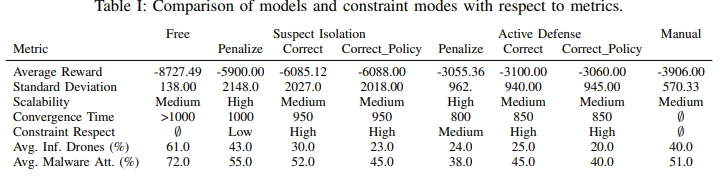
\includegraphics[width=0.5\linewidth]{figures/cage_own_results.png}
  \end{textblock*}

  \begin{textblock*}{14cm}(7.5cm,4.8cm)
    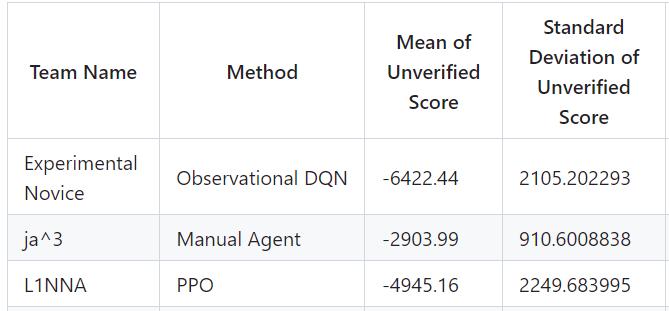
\includegraphics[width=0.5\linewidth]{figures/cage_leader_results.png}
  \end{textblock*}

\end{frame}

\begin{frame}{Cas d'application}{\textbf{K8s Attack/Defense}}

  \centering
  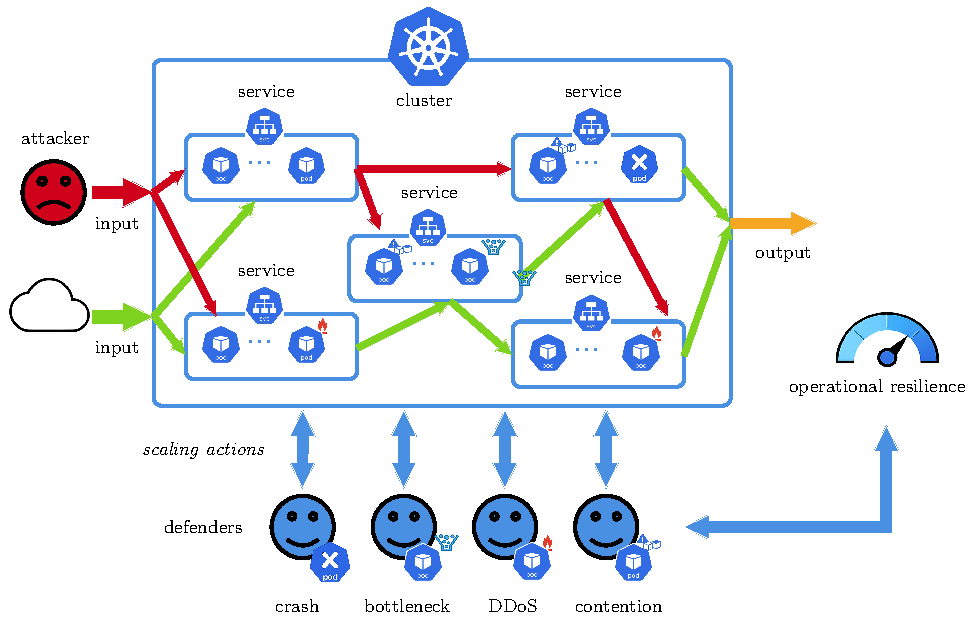
\includegraphics[width=0.8\linewidth]{figures/scenario_introduction.pdf}

\end{frame}

\begin{frame}{Cas d'application}{\textbf{K8s Attack/Defense}}


  \begin{columns}[c]

    \begin{column}{0.4\textwidth}

      \textbf{Approche SMA}
      \begin{itemize}
        \item Un agent par problème
        \item Cibler les problèmes par priorité
        \item Passage à l'échelle facilité
      \end{itemize}

      \

      \textbf{Mise en œuvre dans KARMA}
      \begin{itemize}
        \item PoC fonctionnel sur cluster simple
        \item Amélioration résilience opérationnelle
        \item Convergence plus rapide
      \end{itemize}

    \end{column}

    \begin{column}{0.7\textwidth}

      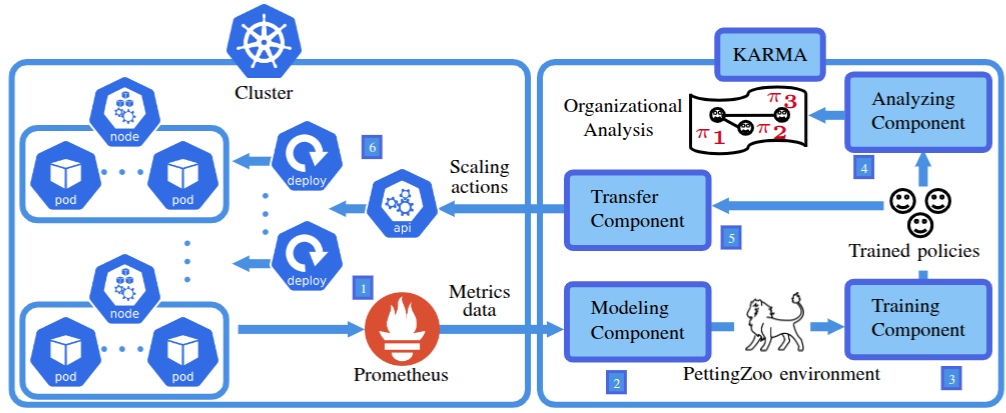
\includegraphics[width=\linewidth]{figures/KARMA_architecture.png}

    \end{column}
  \end{columns}

  \vfill

  {\tiny \begin{spacing}{0.8}
      \textit{J. Soule, J.-P. Jamont, M. Occello, L.-M. Traonouez, and P. Théron. Streamlining Resilient Kubernetes Autoscaling with Multi-Agent Systems via an Automated Online Design Framework. Proceedings of the 18th IEEE International Conference on Cloud Computing (CLOUD), Helsinki, Finland, July 2025. (Accepted).}
    \end{spacing}}

\end{frame}

\section{Conclusion}

\begin{frame}{Conclusion et perspectives}

  \begin{itemize}
    \item Une méthode de conception d'un SMA de Cyberdéfense
    \item Application sur études de cas
    \item[ ] \phantom{X}
    \item \textbf{Travaux courants / futurs}
          \begin{itemize}
            \item Consolidation travaux existants
            \item Rédaction manuscrit, finalisation articles
          \end{itemize}
    \item \textbf{Perspectives}
          \begin{itemize}
            \item Diminution écart \textquote{Simulation - Réalité}
            \item Spécifications organisationnelles dynamiques
            \item Amélioration post-analyse
            \item Ouverture industrielle pour AICA
          \end{itemize}
  \end{itemize}

\end{frame}

\appendix
%\setbeamertemplate{headline}{}
\setbeamertemplate{mini frames}{}

% \AtBeginSection[]{
% 	\begin{frame}
% 		\frametitle{}
% 		\tableofcontents[currentsection]
% 	\end{frame}
% }

% %%%%%%%%%%%%%%%%%%%%%%%%%%%%%%%%%%%%

\section*{\phantom{Thanks}}

\begin{frame}{}

  \vspace{6ex}

  \centering
  {
    \Huge
    \emph{Thank You}
  }

  \vspace{6ex}

  \begin{columns}

    \hspace{-27ex}

    \begin{column}{0.5\textwidth}
      \raggedleft
      {\Large Demo video $\Longrightarrow$}
    \end{column}

    \hspace{-12ex}

    \begin{column}{0.5\textwidth}
      
\includegraphics[width=0.5\linewidth]{figures/demo_qr_code.png}
    \end{column}

  \end{columns}

  \vspace{3ex}

  \centering
  {\Large
    \url{https://t.ly/4JBxr}
  }

\end{frame}


\section*{\phantom{References}}
\begin{frame}[allowframebreaks]{References}{}
  \printbibliography
\end{frame}

\newcounter{mainframenumber}
\setcounter{mainframenumber}{\value{framenumber}}

% % \begin{frame}[allowframebreaks]{Annexes} {Contexte}

    \begin{block}{Paradigme des Systèmes Multi-Agents (SMA) pour des problèmes complexes et distribués}
        \begin{itemize}
            \item \textbf{décomposition des tâches} : missions déléguées aux agents réalisées par coopération~\parencite{Raileanu2023} ;
            \item \textbf{avantages} : gérer des objectifs contradictoires, calcul parallèle, robustesse du système, évolutivité\dots
        \end{itemize}
    \end{block}
    
    \begin{block}{\textbf{Organisation} : clé pour la conception des SMA}
        \begin{itemize}
            \item \textbf{coordination} : comment atteindre un objectif commun de manière collaborative~\parencite{Hubner2007} ;
            \item \textbf{environnements dynamiques et incertains} : comportement flexible à l'exécution pour s'adapter~\parencite{Kathleen2020} ;
        \end{itemize}
    \end{block}
    
    \begin{block}{Méthodes et pratiques pour la conception des SMA}
        \begin{itemize}
            \item \textbf{approche + modèle organisationnel} : les méthodes s'appuient sur l'expérience des concepteurs pour concevoir manuellement les \textbf{politiques} des agents afin que le SMA atteigne ses objectifs ;
                  %   \begin{itemize}
                  %       \item Exemples : \emph{GAIA}~\parencite{Wooldridge2000,Cernuzzi2014}, \emph{ADELFE}~\parencite{Mefteh2015}, ou \emph{DIAMOND}~\parencite{Jamont2015}, \emph{KB-ORG}~\parencite{Sims2008}
                  %   \end{itemize}
            \item \textbf{simulation vers la réalité} : 1) conception sûre et efficace des SMA dans un environnement simulé à haute fidélité ; \quad 2) transfert à un environnement réel pour des performances adéquates~\parencite{Schon2021}.
        \end{itemize}
        \quad $\Longrightarrow$ \textbf{Processus itératif par essais et erreurs}
    \end{block}

\end{frame}

\begin{frame}[allowframebreaks]{Annexes} {Fondamentaux des SMA}

    \begin{block}{Mots-clés}
        \begin{itemize}
            \item \textbf{Agent} : entité immergée dans un environnement, percevant des observations et prenant des décisions de manière autonome pour atteindre des objectifs ;
            \item \textbf{SMA} : ensemble d'agents collaborant avec des mécanismes d'auto/réorganisation pour atteindre leurs objectifs ;
            \item \textbf{Organisation} : interactions des agents même si elles peuvent être implicites ;
            \item \textbf{Modèle organisationnel (OM)} : moyen de décrire formellement une organisation explicite/implicite ;
            \item \textbf{Spécifications organisationnelles (OS)} : composants d'un OM pour caractériser une organisation.
        \end{itemize}
    \end{block}
    
    \begin{block}{Modèle organisationnel : $\mathcal{M}OISE^+$}
        \begin{itemize}
            \item plus complexe que \emph{Agent Group Roles} (intégration des normes) ;
            \item prend explicitement en compte les aspects sociaux entre les agents ;
            \item permet de lier les politiques des agents aux spécifications organisationnelles.
        \end{itemize}
    \end{block}

\end{frame}

\begin{frame}[allowframebreaks]{Annexes} {Fondamentaux du MARL}

    \begin{block}{Mots-clés}
        \begin{itemize}
            \item \textbf{Politique} : la \textquote{logique} pour choisir la prochaine action en fonction de l'observation pour un agent ;
            \item \textbf{Historique/trajectoire} : le couple (observation, action) sur un épisode ;
            \item \textbf{Politique/historique conjoints} : l'ensemble des politiques/historiques de tous les agents sous forme de tuples ;
            \item \textbf{Apprentissage par renforcement} : un agent met à jour sa politique pour maximiser une récompense cumulative ;
            \item \textbf{Apprentissage par renforcement multi-agent (MARL)} : extension à plusieurs agents qui apprennent en prenant en compte les actions des autres agents ;
        \end{itemize}
    \end{block}
    
\end{frame}

\begin{frame}[allowframebreaks]{Annexes}{Approche AOMEA : Fondement théorique}
    \begin{block}{MARL orienté organisation (OMARL)}
        Un processus de MARL augmenté avec un OM pour :
        \begin{itemize}
            \item \textbf{Contraindre l'espace des politiques} : obtenir les politiques conjointes satisfaisant les spécifications de conception données ;
            \item \textbf{Inférer des spécifications organisationnelles} : obtenir des spécifications à partir des politiques des agents.
        \end{itemize}
    \end{block}
    
    \begin{block}{Algorithme \emph{Partial Relations with Agent History and Organization Model} (PRAHOM)}
        Implémentation d'un processus OMARL\dots
        \begin{enumerate}
            \item \textbf{Contraindre l'espace des politiques}
                  \begin{itemize}
                      \item Impossible d'utiliser directement les politiques $\rightarrow$ \textbf{historiques} caractérisant les \textbf{politiques} ;
                      \item Relations entre \textbf{OS} et historiques attendus ;
                      \item Les agents contraints aux OS $\rightarrow$ à chaque étape : actions disponibles mises à jour en fonction des historiques \textbf{OS}.
                  \end{itemize}
    
            \item \textbf{Inférer des spécifications organisationnelles}
                  \begin{itemize}
                      \item Analyser les historiques $\rightarrow$ caractériser les comportements collectifs comme OS ;
                      \item Utilisation des relations connues entre OS et historiques ;
                      \item Utilisation de la définition générale des OS par rapport aux historiques.
                  \end{itemize}
        \end{enumerate}
    \end{block}
    
\end{frame}

\begin{frame}{Annexes}{Aperçu de \textit{PRAHOM}}
    \begin{figure}
        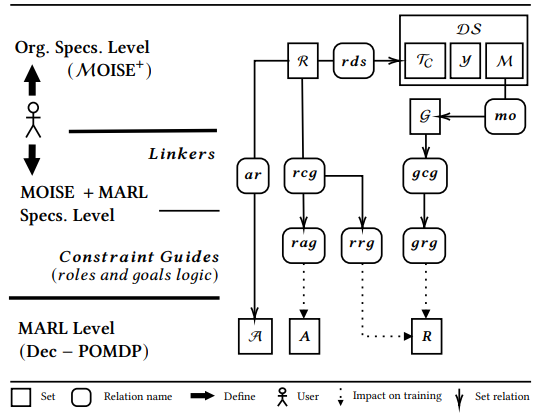
\includegraphics[width=0.6\linewidth]{figures/mm_simple_representation.png}
    \end{figure}
\end{frame}
    
\begin{frame}{Annexes}{Aperçu de PRAHOM}
    \begin{figure}
        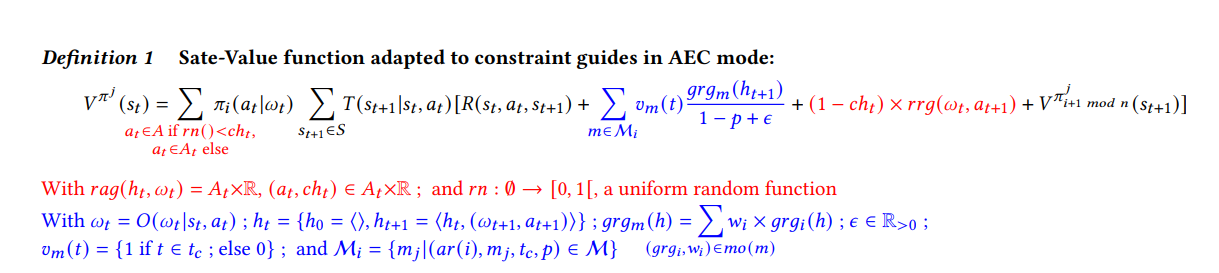
\includegraphics[width=\linewidth]{figures/modified_state_value_function.png}
    \end{figure}
\end{frame}
    
\begin{frame}[allowframebreaks]{Annexes}{Approche AOMEA : Fondement théorique}
    \textbf{Contraindre l'espace des politiques} pendant l'entraînement

    \begin{columns}
    
        \begin{column}{0.3\textwidth}
    
            \begin{itemize}
                \item À chaque étape, l'ensemble des actions disponibles est modifié pour correspondre aux contraintes de politiques définies par les utilisateurs ;
                \item Contraintes intégrées via : correction externe, apprentissage, modification interne des politiques.
            \end{itemize}
    
        \end{column}
    
        \begin{column}{0.8\textwidth}
            \begin{figure}
                \centering
                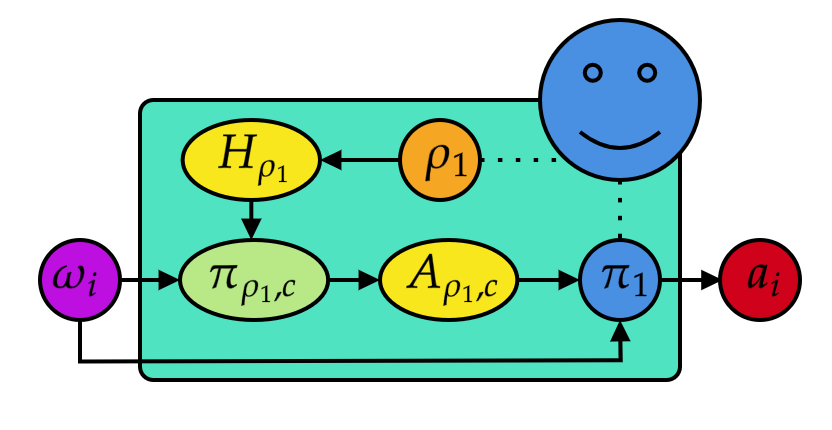
\includegraphics[width=0.7\linewidth]{figures/prahom_training_constrain.png}
                \caption*{Vue résumée de la contrainte PRAHOM}
                \label{fig:prahom_process}
            \end{figure}
        \end{column}
    
    \end{columns}
\end{frame}

\begin{frame}{Annexes}{Constrained Reinforcement Learning (Constrained-RL)}
    
    \begin{itemize}
        \item Apprendre une politique optimisant la récompense tout en respectant des \textbf{contraintes de sécurité} ou de \textbf{performance}.
        
        \item \textbf{Contraintes dures} : doivent toujours être respectées (Shielding).
        \item \textbf{Contraintes douces} : respectées en moyenne ou sous forme de pénalités.
        
        \item \textbf{Méthodes :}
            \begin{itemize}
                \item \textbf{Reward Shaping} : ajout de pénalités pour violation de contraintes.
                \item \textbf{Policy Projection} : ajustement des actions pour rester dans les limites.
                \item \textbf{Dual Variables} : intégration de multiplicateurs de Lagrange pour gérer les contraintes.
            \end{itemize}
            
    \end{itemize}    
\end{frame}

\begin{frame}{Annexes}{Safe Exploration et Shielding en Reinforcement Learning}
    
    \begin{itemize}
        \item \textbf{Safe Exploration} $\rightarrow$ garantir la sécurité lors de la phase d'exploration en limitant les risques de comportements dangereux.
        \item Principalement modifier la fonction de récompense (Langragien) pour integrer contraintes mais aussi\dots
        \item \textbf{Shielding} intervenir en temps réel pour bloquer les actions susceptibles de violer ces contraintes, permettant une exploration sécurisée.
    \end{itemize}
    
    \textbf{Référence :} \\
    \textit{Akifumi Wachi, Wataru Hashimoto, Xun Shen, \& Kazumune Hashimoto (2023). Safe Exploration in Reinforcement Learning: A Generalized Formulation and Algorithms. In Thirty-seventh Conference on Neural Information Processing Systems.}

\end{frame}

\begin{frame}[allowframebreaks]{Annexes}{Approche AOMEA: Fondement théorique}

    \textbf{Inferrer des Spécifications Organisationnelles}

    \begin{columns}

        \begin{column}{0.3\textwidth}

            \begin{itemize}
                \item \textbf{Knowledge-based Organizational Specifications Identification (KOSIA)}
                \item \textbf{General Organizational Specifications Infererence (GOSIA)}
            \end{itemize}

        \end{column}

        \begin{column}{0.8\textwidth}
            \begin{figure}
                \centering
                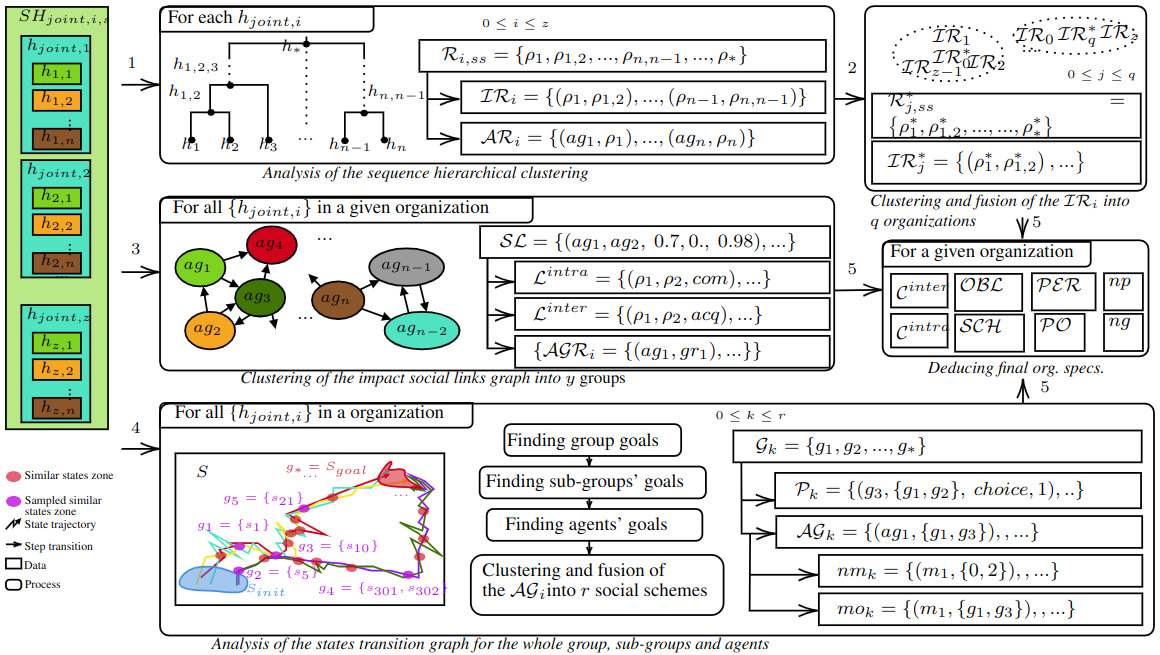
\includegraphics[width=0.95\linewidth]{figures/GOSIA_view.png}
                \caption*{A summary view of the GOSIA process}
                \label{fig:gosia_process}
            \end{figure}
        \end{column}

    \end{columns}

\end{frame}


%%%%%%%%%%%%%%%%

% Slide 2: Exemple d'utilisation
\begin{frame}[fragile]{Annexes}{Exemple d'utilisation d'Optuna}
    \begin{itemize}
        \item \textbf{Optuna} est une bibliothèque open-source pour l'optimisation des hyperparamètres (HPO), utile en apprentissage automatique.
        \item Exemples d'hyper-paramètre : taux d'apprentissage, fonction activation, nb couche, taille couches, seuil de ressemblance pour Hierarchical Clustering\dots
        \item \textbf{Étapes pour utiliser Optuna :}
        \begin{itemize}
            \item \texttt{1.} Définir une fonction d'objectif.
            \item \texttt{2.} Lancer une étude avec Optuna.
            \item \texttt{3.} Utiliser le meilleur résultat pour entraîner le modèle.
        \end{itemize}
    \end{itemize}

    \begin{lstlisting}[language=Python, basicstyle=\small\ttfamily, frame=single, caption=Exemple d'Optuna en Python]
import optuna

def objective(trial):
    x = trial.suggest_float("x", -10, 10)
    return (x - 2) ** 2 # Mock : fonction "etat-valeur"

study = optuna.create_study(direction="minimize")
study.optimize(objective, n_trials=100)

print(study.best_params)  # Affiche les meilleurs parametres
    \end{lstlisting}
\end{frame}


\begin{frame}{Annexes}{Aperçu PettingZoo}
    \begin{itemize}
        \item Bibliothèque Python pour environnements multi-agents.
        \item Simplifier l'entraînement et l'évaluation des agents dans divers environnements.
        \item \textbf{Caractéristiques principales} :
        \begin{itemize}
            \item Supporte plusieurs types d'environnements multi-agents (tour par tour, simultané, etc.).
            \item Intégration facile avec des frameworks de reinforcement learning comme RLlib.
            \item Compatible avec les API de Gym, permettant une utilisation intuitive.
        \end{itemize}
        \item \textbf{Exemples d'environnements inclus} :
        \begin{itemize}
            \item Jeux : \textit{TicTacToe}, \textit{ConnectFour}.
            \item Scénarios de collaboration et de compétition : \textit{Pistonball}, \textit{Prisoner's Dilemma}.
            \item Intégration avec la suite d'environnements Atari pour le multi-agent.
        \end{itemize}
    \end{itemize}
\end{frame}

\begin{frame}[fragile]{Annexes}{Exemple utilisation de PettingZoo}
    \begin{itemize}
        \item Exemple : Création et interaction avec un environnement.
        \item Chargement de l'environnement, réinitialisation et étapes d'interaction pour un agent.
    \end{itemize}
    \vspace{0.3cm}
    \begin{lstlisting}[language=Python, basicstyle=\ttfamily\small]
from pettingzoo.butterfly import pistonball_v6

# Creer et reinitialiser l'environnement
env = pistonball_v6.env()
env.reset()

# Boucle principale d'interaction
for agent in env.agent_iter():
    obs, reward, done, info = env.last()
    action = env.action_space(agent).sample()  # Action aleatoire
    env.step(action)
    if done:
        env.reset()  # Reinitialiser si l'episode est termine
\end{lstlisting}
\end{frame}


\begin{frame}{Annexes}{KB-Org}
    \frametitle{Organization-based multi-agent systems: From modeling to implementation}
    
    \begin{itemize}
        \item Modélisation et mise en œuvre des SMA basés sur organisation ;
        \item Intègre les concepts d'organisation pour structurer les interactions et le comportement des agents ;
        \item Banque d'organisations disponibles prêtes à être utilisé ;
        \item Explicabilité et à la coordination.
    \end{itemize}
    
    \

    Sims, V. (2008). Automated organization design for multi-agent systems. Autonomous Agents and Multi-Agent Systems, 16(2), 151-185.

\end{frame}

\begin{frame}{Annexes}{Présentation de la bibliothèque MARLlib}

    \begin{itemize}
        \item Bibliothèque Python pour MARL
        \item Supporte plusieurs environnements MARL comme PettingZoo, StarCraft II, MPE (Multi-Agent Particle Environment), etc.
        \item Implémente divers algorithmes MARL, incluant MADDPG, MAPPO, etc.
        \item Fournit une interface pour comparaison d’algorithmes, l’entraînement et l’évaluation.
        \item Offre des configurations \textit{fine-tunés} pour de nombreux environnements
    \end{itemize}

\end{frame}

\begin{frame}[allowframebreaks]{Annexes}{Présentation de la bibliothèque MARLlib}

    \begin{itemize}
        \item \textbf{Algorithmes Basés sur les Valeurs}  
        \begin{itemize}
            \item \textbf{Multi-Agent Q-Learning} : Une extension multi-agent fondamentale de Q-learning.  
            \textit{Description} : Simple à implémenter, mais avec des difficultés de scalabilité et de non-stationnarité.
            \item \textbf{MADDPG} : Une adaptation de DDPG pour les environnements multi-agents.  
            \textit{Description} : Gère bien les espaces d'actions continues, mais requiert beaucoup de données et est complexe.
        \end{itemize}
    
        \

        \item \textbf{Algorithmes Basés sur les Politiques}  
        \begin{itemize}
            \item \textbf{REINFORCE} : Une méthode de gradient de politique basique pour l'apprentissage direct de la politique.  
            \textit{Description} : Adaptable aux environnements stochastiques mais souffre de variances élevées des gradients.
            \item \textbf{Multi-Agent PPO (MAPPO)} : Une extension de PPO conçue pour les configurations multi-agents.  
            \textit{Description} : Stabilise les mises à jour, mais nécessite un ajustement minutieux et un coût de calcul élevé.
        \end{itemize}
    
        \item \textbf{Algorithmes Hybrides}  
        \begin{itemize}
            \item \textbf{A3C (Asynchronous Advantage Actor-Critic)} : Combine l'apprentissage des politiques et des valeurs pour un équilibre exploration/exploitation.  
            \textit{Description} : Accélère l'entraînement mais nécessite une synchronisation complexe.
            \item \textbf{MAPPO} : Un hybride intégrant PPO avec un entraînement centralisé.  
            \textit{Description} : Efficace pour les tâches coopératives, mais difficile dans les environnements compétitifs et exigeant en ressources.
        \end{itemize}
    
        \item \textbf{Algorithmes Théoriques et Coopératifs Basés sur le Jeu}  
        \begin{itemize}
            \item \textbf{Independent Q-Learning (IQL)} : Une version indépendante de Q-learning pour chaque agent.  
            \textit{Description} : Simple à implémenter mais avec de sérieux problèmes de non-stationnarité en multi-agent.
            \item \textbf{COMA (Counterfactual Multi-Agent Policy Gradients)} : Utilise des baselines contrefactuelles pour évaluer les contributions des agents.  
            \textit{Description} : Réduit la variance et améliore la coopération, mais demande des calculs lourds.
        \end{itemize}
    
        \item \textbf{Entraînement Centralisé avec Exécution Décentralisée}  
        \begin{itemize}
            \item \textbf{QMIX} : Décompose les valeurs Q pour améliorer la coordination multi-agent.  
            \textit{Description} : Équilibre l'entraînement centralisé et l'action décentralisée, mais moins efficace en environnements très compétitifs.
            \item \textbf{VDN (Value Decomposition Networks)} : Simplifie la coordination multi-agent avec la décomposition des valeurs.  
            \textit{Description} : Efficace mais limité dans la gestion d'interactions complexes.
        \end{itemize}
    \end{itemize}
    

\end{frame}


\end{document}
